\chapter{Benchmarking}
\label{sec:benchmarking}

In this section we evaluate the performance of the Reo-rs library, focusing primarily on the optimizations described in Section~\ref{sec:protocol_runtime}.

\section{Experimental Setup}

this kind of machine blah blah.

we have a number of tests with these conditions:

\begin{enumerate}
	\item \textbf{Reo overhead}\\
	TODO
	
\end{enumerate}



%\begin{landscape}
%\begin{table}[p!]
%\begin{adjustbox}{width=19cm}
%\rowcolors{2}{gray!13}{white}
%\begin{tabular}{l|ll|p{46mm}p{67mm}}
%\rowcolor{gray!26}
%Name & Connector & Data Type & Goal & Description \\
%
%\hline
%seq-fifo & fifo1 & Integer & Tease out Proto overhead & alternate between putting and getting on single thread. measure RTT. Repeat for different sizes of data. Compare overhead to std::spsc channel \\
%
%SIMO clone & N-replicator & BigClonable & check if getters are effectively cloning in parallel & repeatedly clone from a single putter in parallel \\
%
%SIMO copy & N-replicator & BigCopyable & check if copying saves a lot of time vs cloning & repeatedly copy from a single putter in parallel \\
%
%MO clone & N-keeper & BigClonable & Check if waiting for putter adds significant time & repeatedly clone from a memcell \\
%
%counting & binary counter & BigClonable & Check how effective the refcounting is & binary counter circuit, moving memory between cells a hell of a lot. not much firing \\
%
%MO fine & N-keeper fine & BigClonable & Check if coordinator is the bottleneck & have one rule per getter. each readiness causing a firing. \\
%
%bitsets & N-keeper fine & BigClonable & fire every time, but after N-1 false guard evals by bitsets & N-keeper where only the last port and rule are active. effectively have to traverse all these dead rules each time \\
%
%hashsets & N-keeper fine & BigClonable & check if the bitsets themselves helped & repeat bitset experiments, but modify Reo-rs to use stdlib hashsets instead \\
%
%transform & transformer & int, float & overhead of createfromcall & \\
%
%filter & filter & int & & \\
%
%router & router & int & & \\
%
%parallel & parallel & BitCopyable & concoct a scenario where data is moving in parallel as much as possible. & 
%
%\end{tabular}
%\end{adjustbox}
%\caption[TODO]{TODO}	
%\end{table}
%\end{landscape}

\section{Reo-rs in Context}

\subsection{Versus the Java Implementation}
We begin by making the most intuitive benchmark to get an understanding of how effectively Reo-rs has been optimized for its task; we compare it to the work of the Reo compiler's Java code-generator. This comparison spans two vastly different systems with different goals, but also compare a memory-managed language to a system's language. The reader should bear this in mind when interpreting the measurements. As our test scenario, we have a set of $N$ getters repeatedly copying some memory value $M$, retained inside the protocol from initialization. By involving a contended resource, we are able to test and compare the \textit{scalability} the generated programs, both in terms of number of ports and the size of the transmitted data.

\begin{figure}
	\centering
	\makebox[\textwidth][c]{
		\begin{subfigure}[b]{0.63\textwidth}
			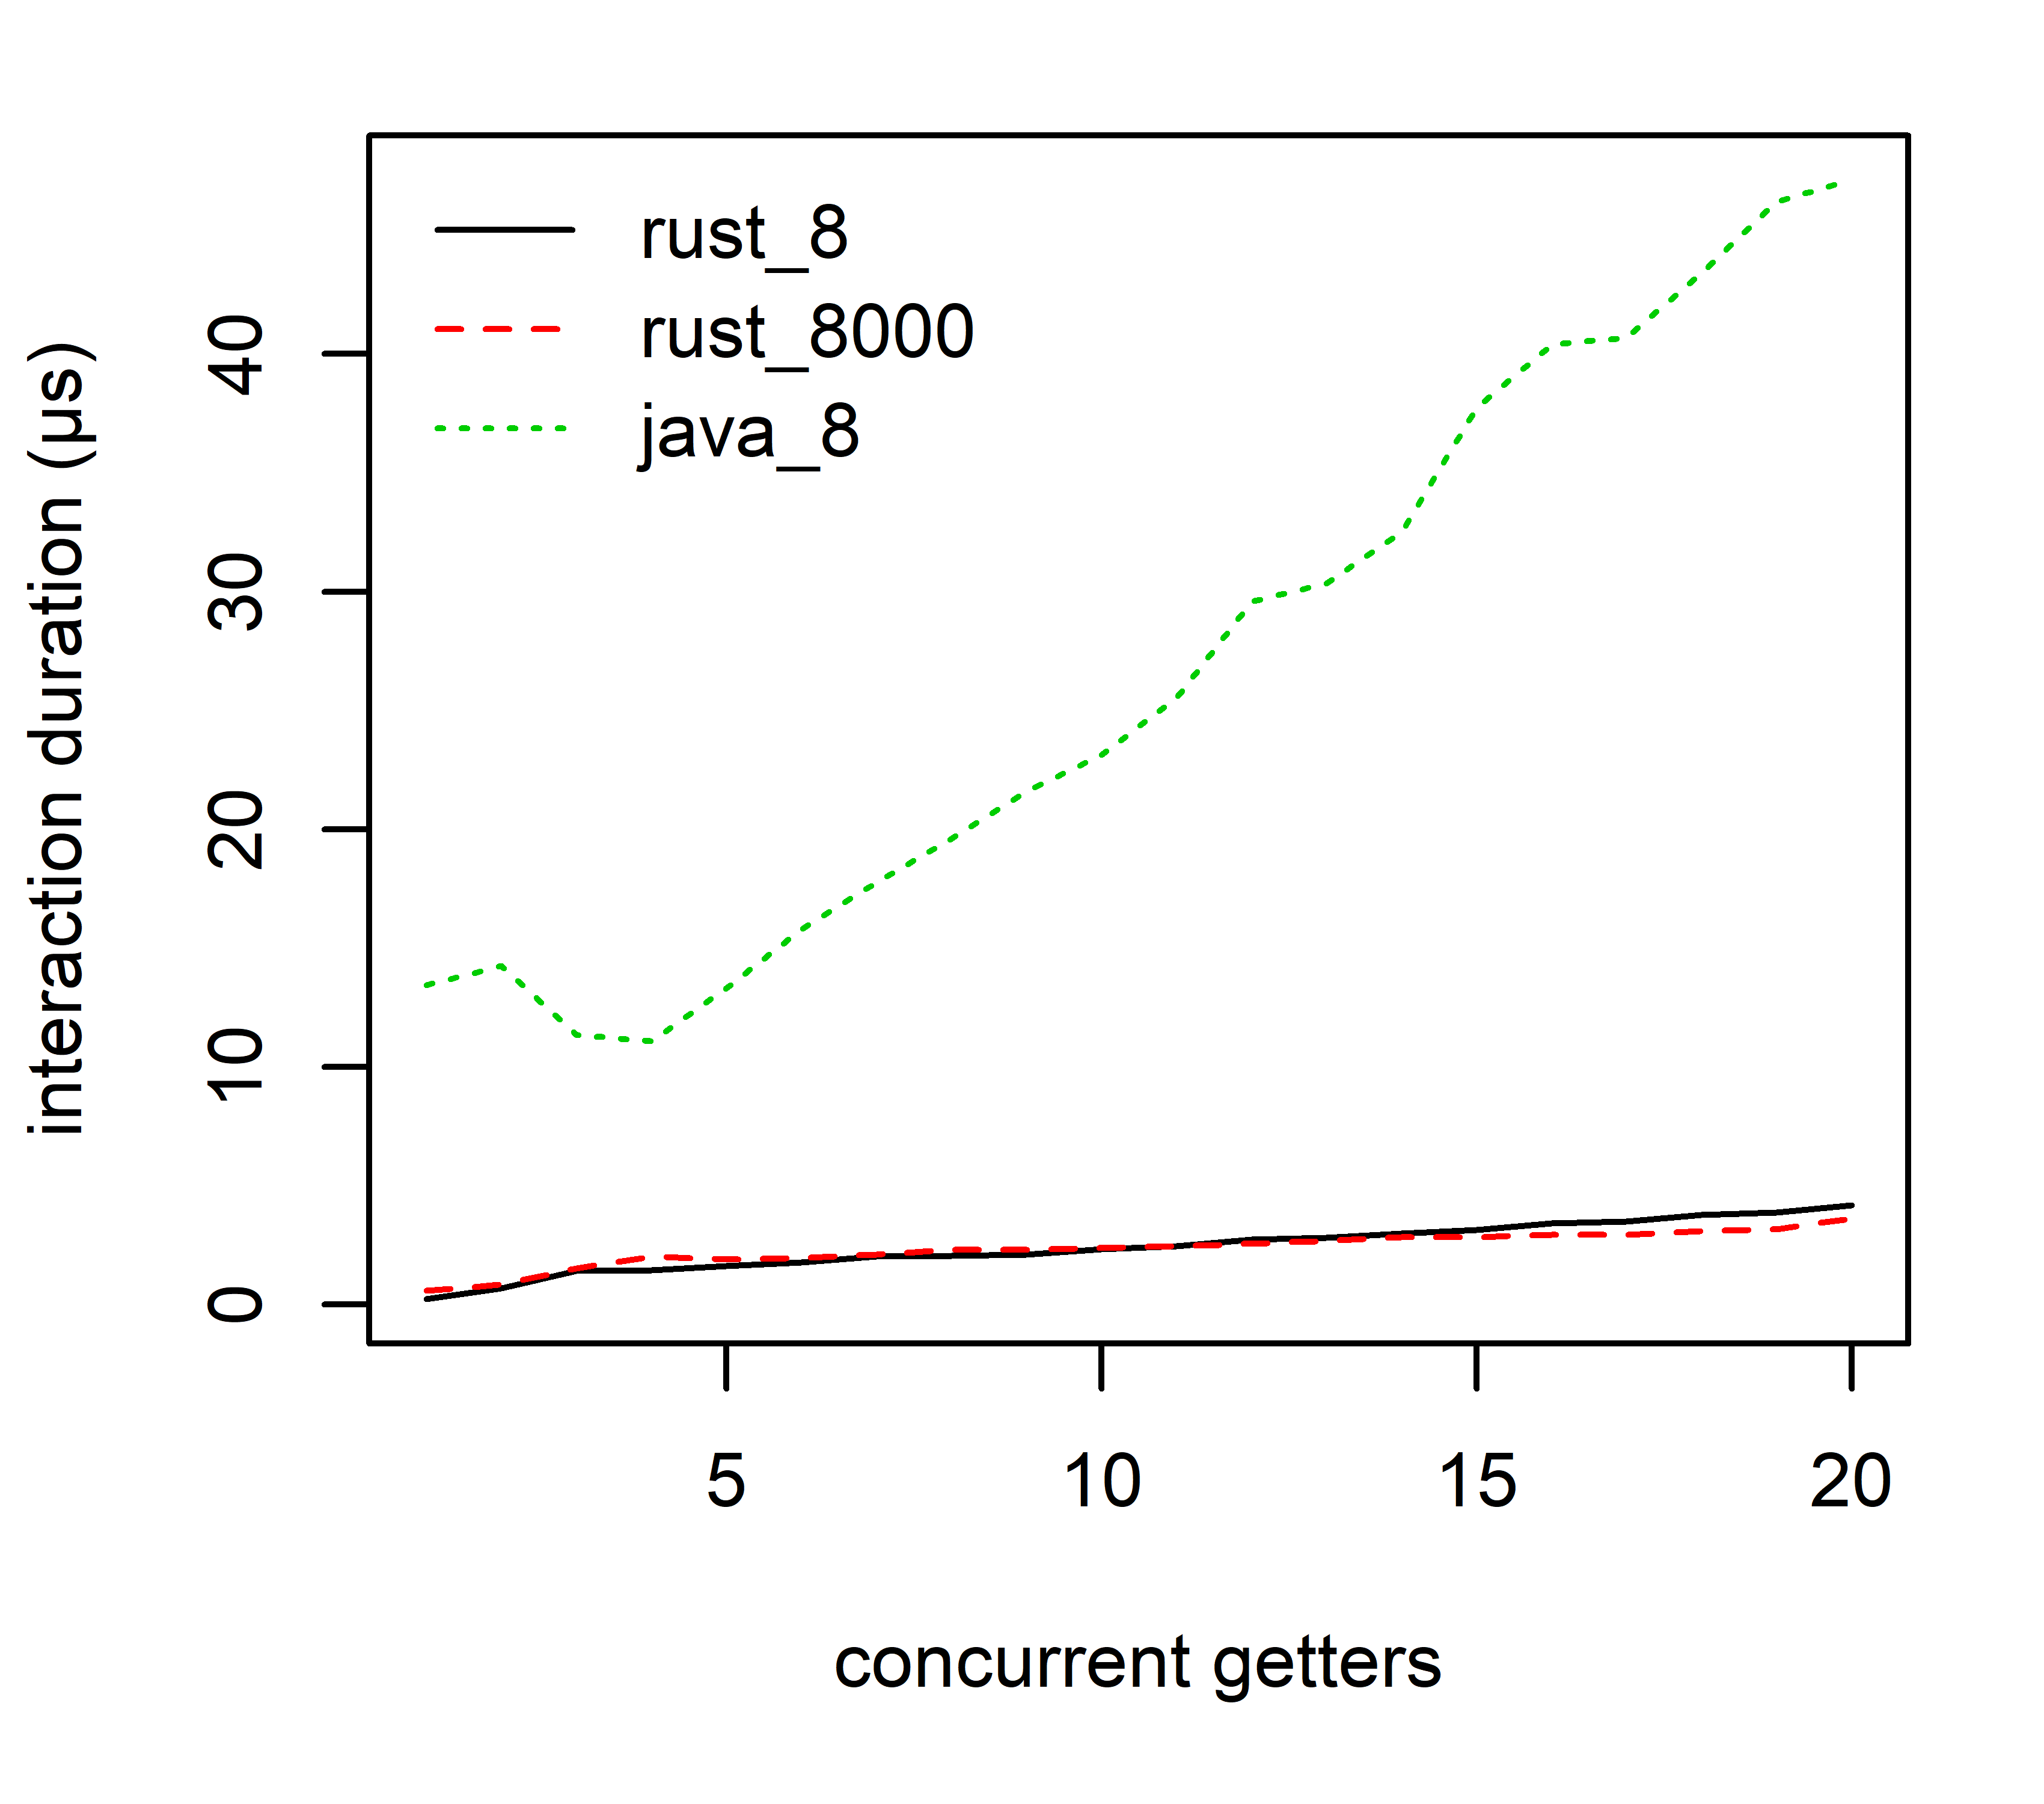
\includegraphics[width=\textwidth]{experiments/rust_v_java_0.png}
			\caption{}
			\label{fig:rust_v_java_0}
		\end{subfigure}%
		\begin{subfigure}[b]{0.63\textwidth}
			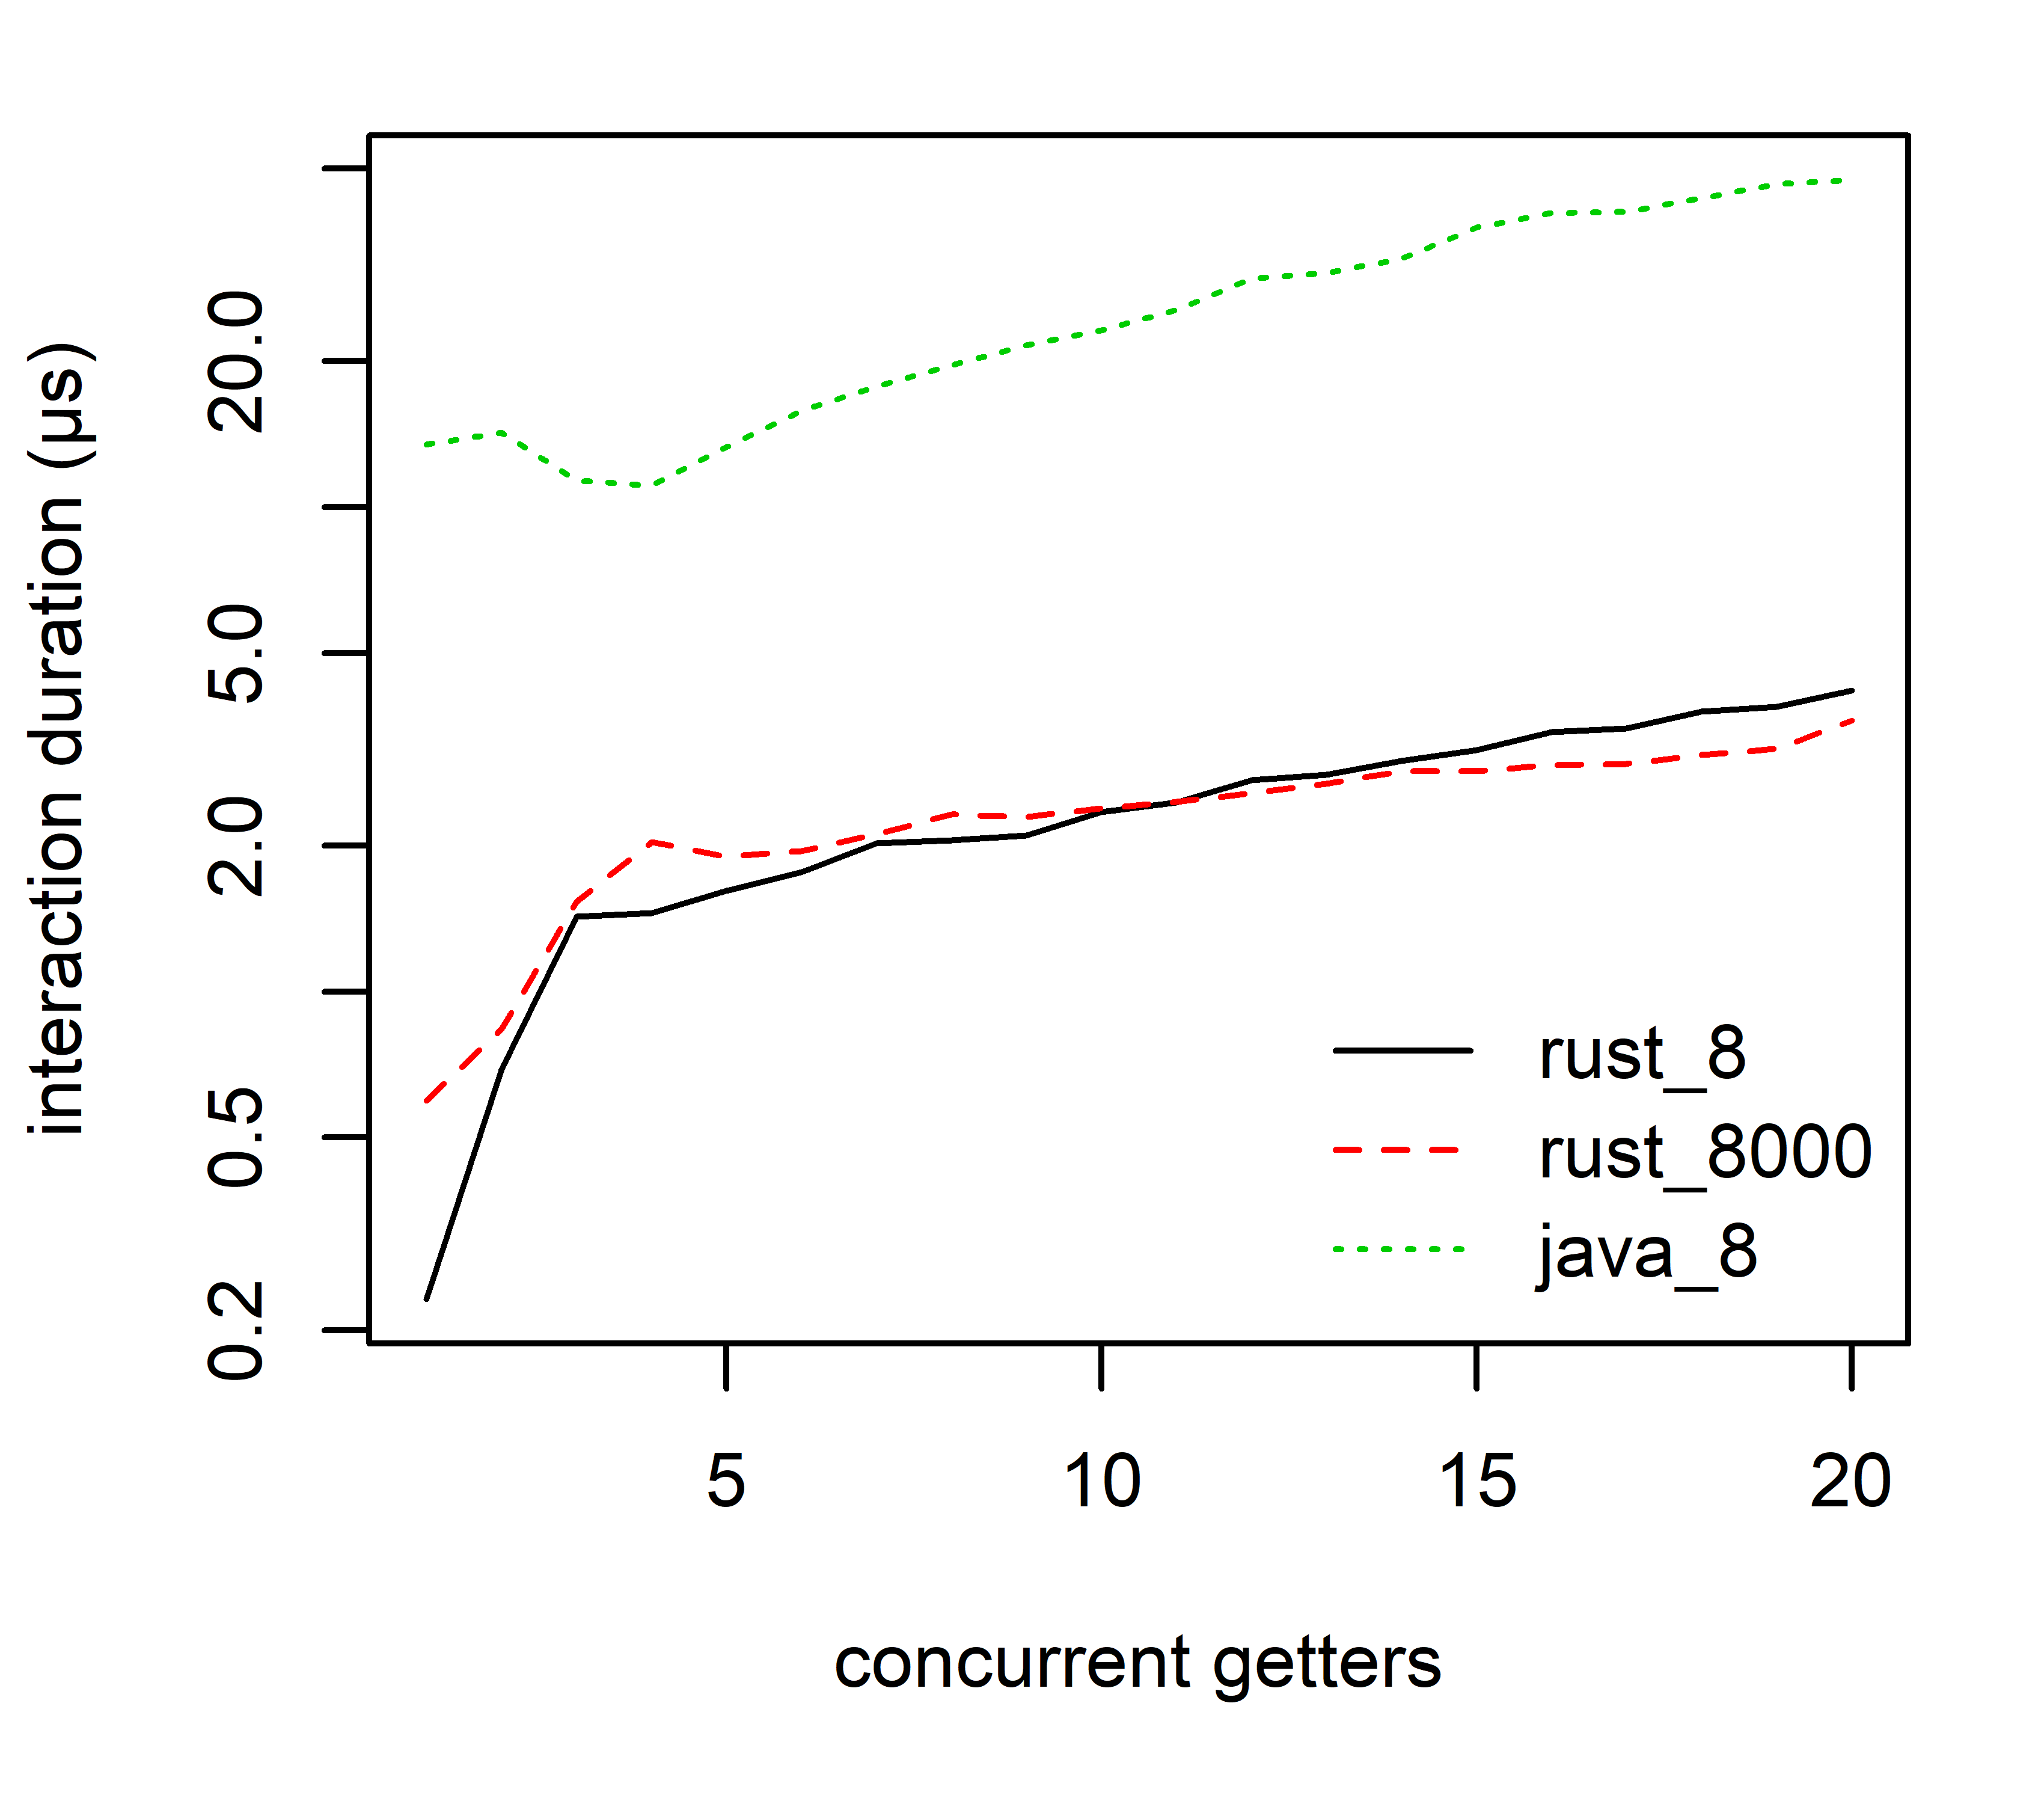
\includegraphics[width=\textwidth]{experiments/rust_v_java_1.png}
			\caption{}
			\label{fig:rust_v_java_1}
		\end{subfigure}%
	}
	\caption[Java vs.\ Rust interaction time for small values.]{Comparison of interaction time for the \textit{fetch} connector for both Java and Rust backends moving small-size values. `rust\_8' and `java\_8' both move a payload of 8~bytes (to match the reference size of the 64-bit JVM). `rust\_8000' gives an example of how the runtime of Reo-rs can change with respect to modest changes in data size. The two sub-figures mirror one another except for the linear and logarithmic y-axes respectively.}
	\label{fig:rust_v_java}
\end{figure}

The unfairness of our comparison cuts both ways, as there is not a clear means of comparing the transmission of large values; the Java version relies entirely on object-aliasing, effectively implementing different semantics. For Java, the size of values transmitted is largely irrelevant. We begin by a comparison on the only common ground; Figure~\ref{fig:rust_v_java_0} shows both Java and Rust are transmitting pointer-sized objects. Aside from the order of magnitude difference in runtime, we observe a different \textit{shape}. Reo-rs is observed to be significantly faster for a single-getter case. This is easy enough to explain; the type relied upon for protecting the coordinator's \textit{critical region} is \code{Mutex} from the \code{parking\_lot} crate, which provides implementations of these kinds of concurrency primitives. \code{Mutex}~is documented as having a \textit{fast path} optimization for when the lock is acquired \textit{uncontested}. Runs with one getter are thus able to take advantage of this optimization every time.

Figure~\ref{fig:rust_v_java_2} attempts to draw the same comparison as before, but in the case of large data-types. The Java-generated protocol objects do not do true value-passing. It is out of the scope of this project to attempt to implement this

\begin{figure}
	\centering
	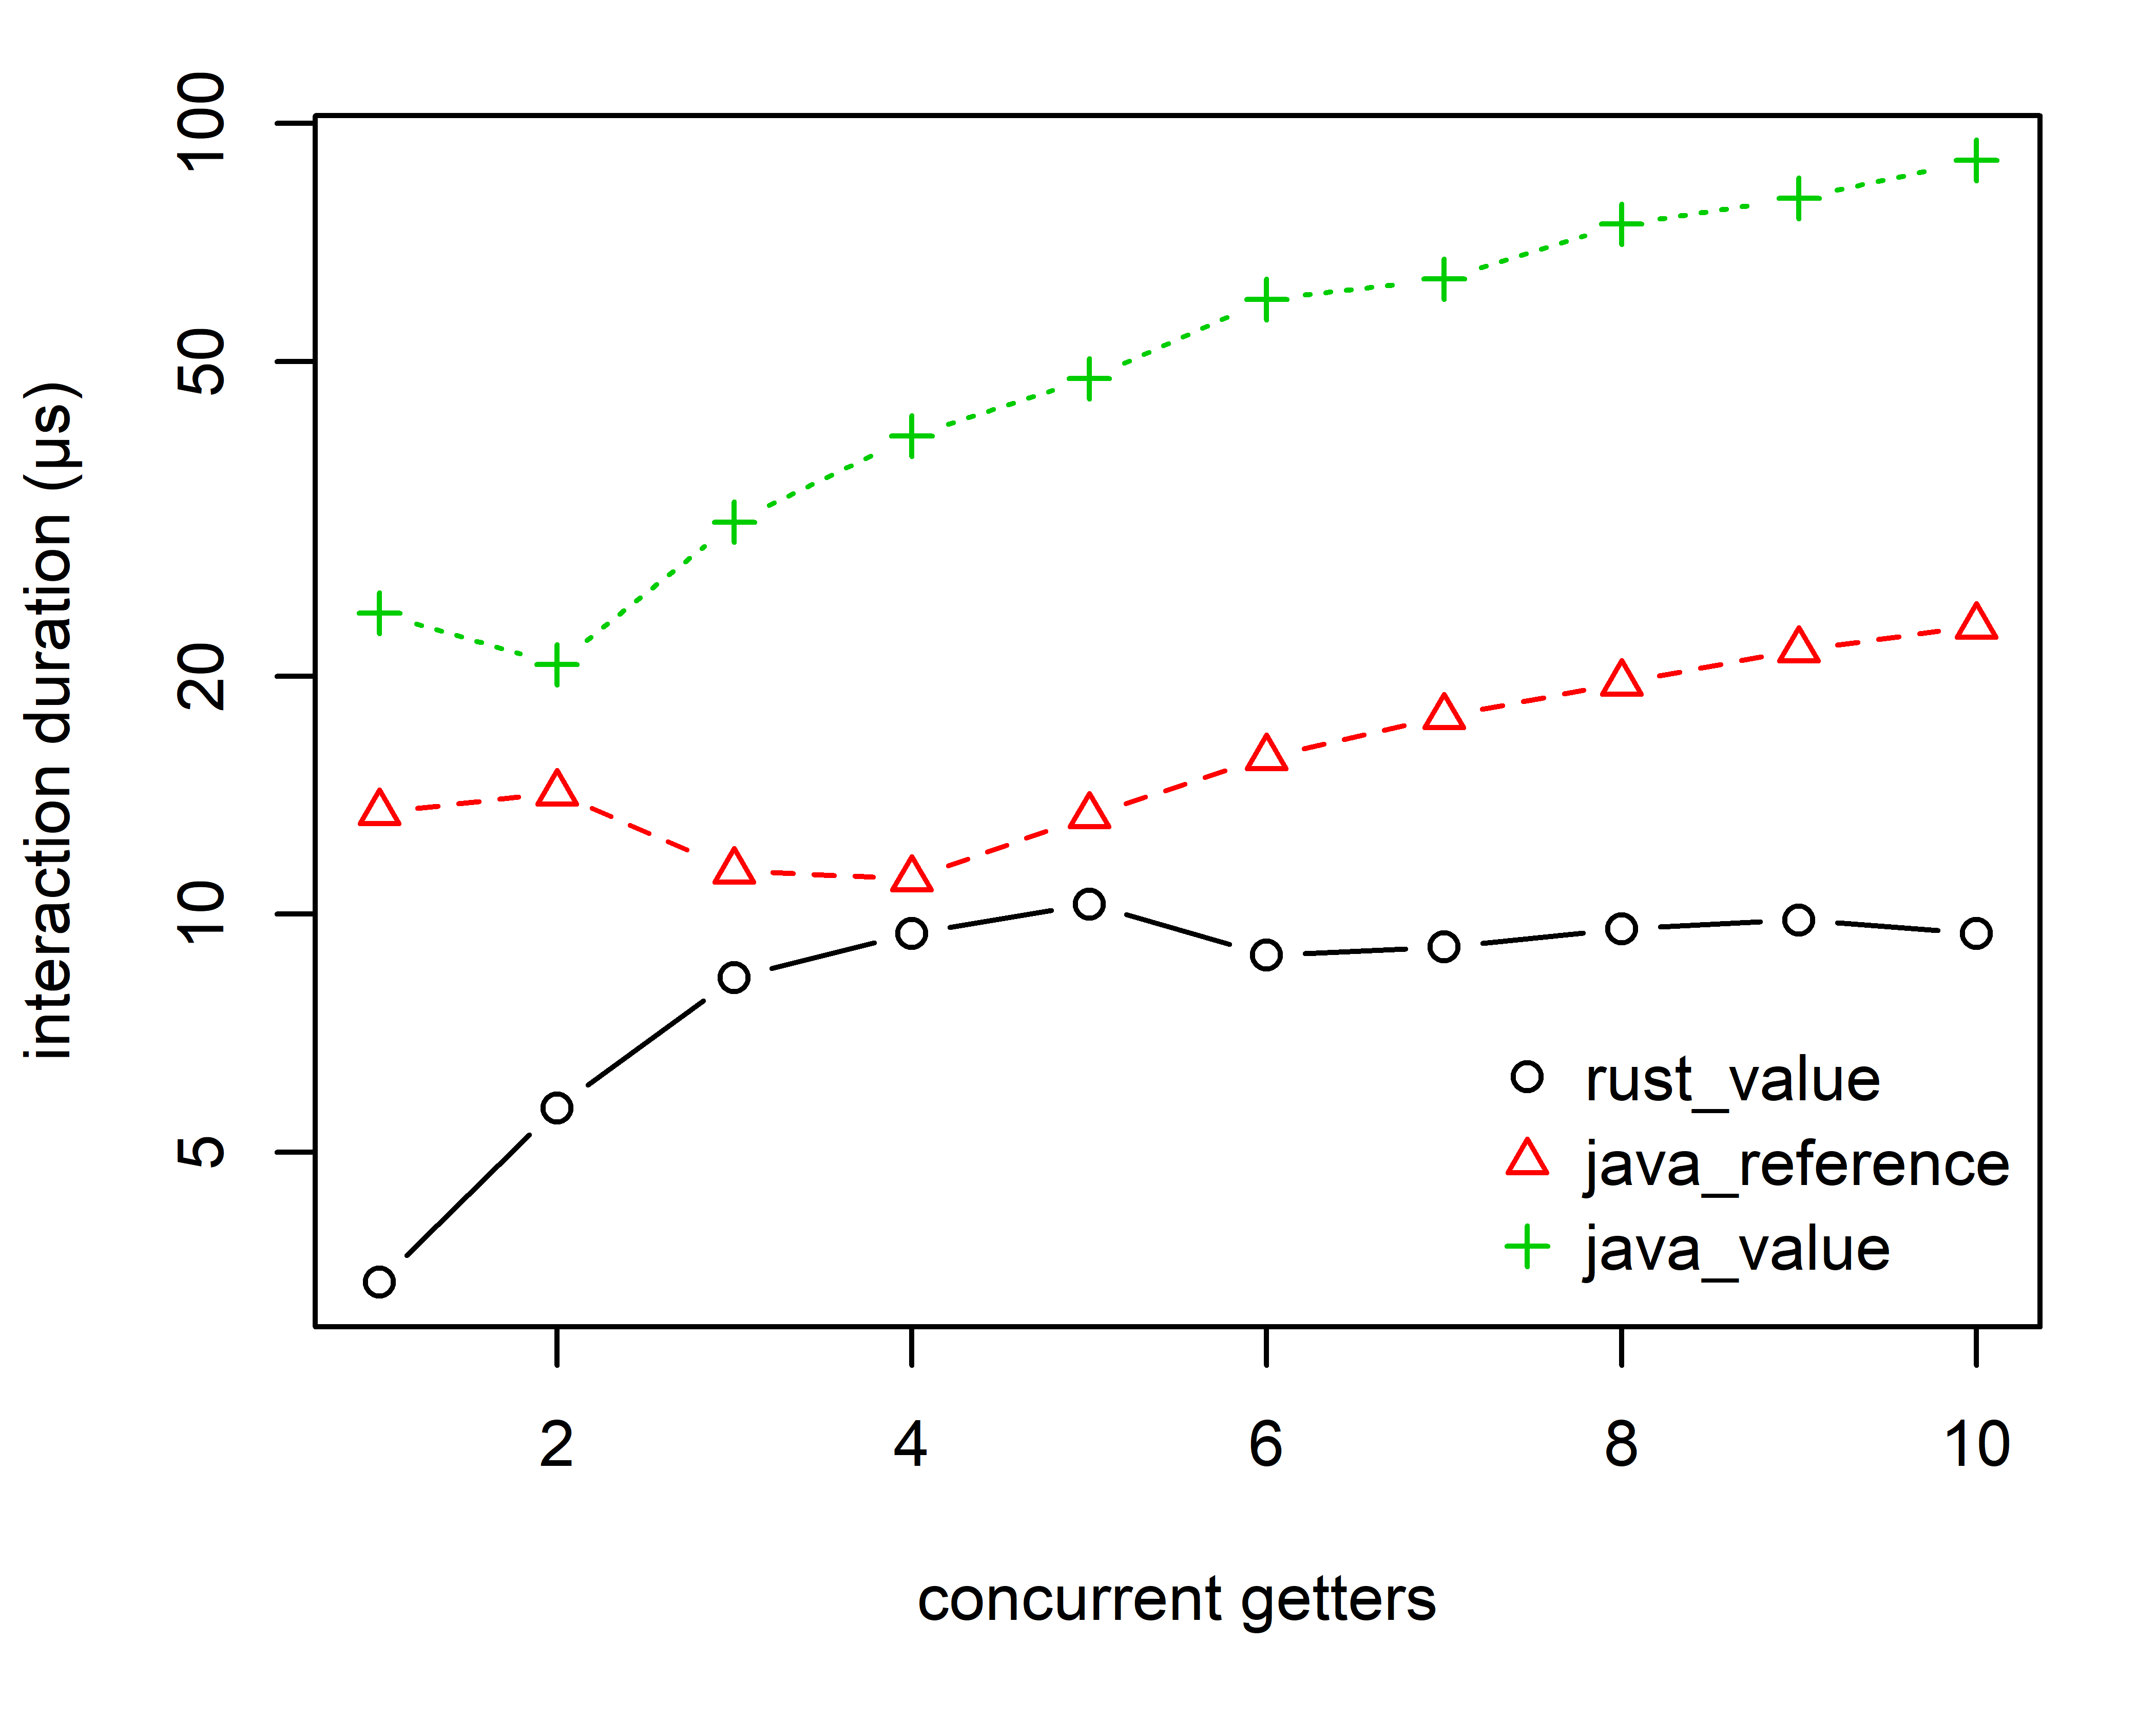
\includegraphics[width=0.80\textwidth]{experiments/rust_v_java_2.png}
	\caption[Java vs.\ Rust interaction time for large values.]{Comparison of interaction time for the \textit{fetch} connector for both Java and Rust backends moving 64-kilobyte-sized data. The Rust backend moves the datum by value, while the Java parallel `java\_reference' aliases the object (moving by reference). This backend does not support semantics-preserving value-passing. We achieve safety here by the coordinator injecting \code{clone} operations of byte arrays to mirror Rust's bit-wise value-copy, called `java\_value'. Note the logarithmic y-axis.}
	\label{fig:rust_v_java_2}
\end{figure}

\subsection{Versus Hand-Crafted Programs}

Ideally, Reo-generated protocol objects would perform precisely the operations we wish without any overhead at all in every situation. However, synchronization does not come for free; lock contention causes overhead (either explicit locks, or hardware-level locks using atomic operations) and bookkeeping takes time. First, we wish to understand the extent to Reo's overhead over the bare-minimal solution for a particular \textit{instance} of protocol: a fifo1 channel. Figure~\ref{fig:exper_rtt} compares the total `round trip time', measuring the mean duration of a `round trip' of a single element, ie.\ starting from the moment \code{put} begins to the moment \code{get} ends. Sub-figure~\ref{fig:exper_rtt_0} shows this in contrast to the simplest channels in Rust's standard library: \code{mpsc} (`multiple producer, single consumer').


\begin{figure}
	\centering
	\makebox[\textwidth][c]{
		\begin{subfigure}[b]{0.63\textwidth}
			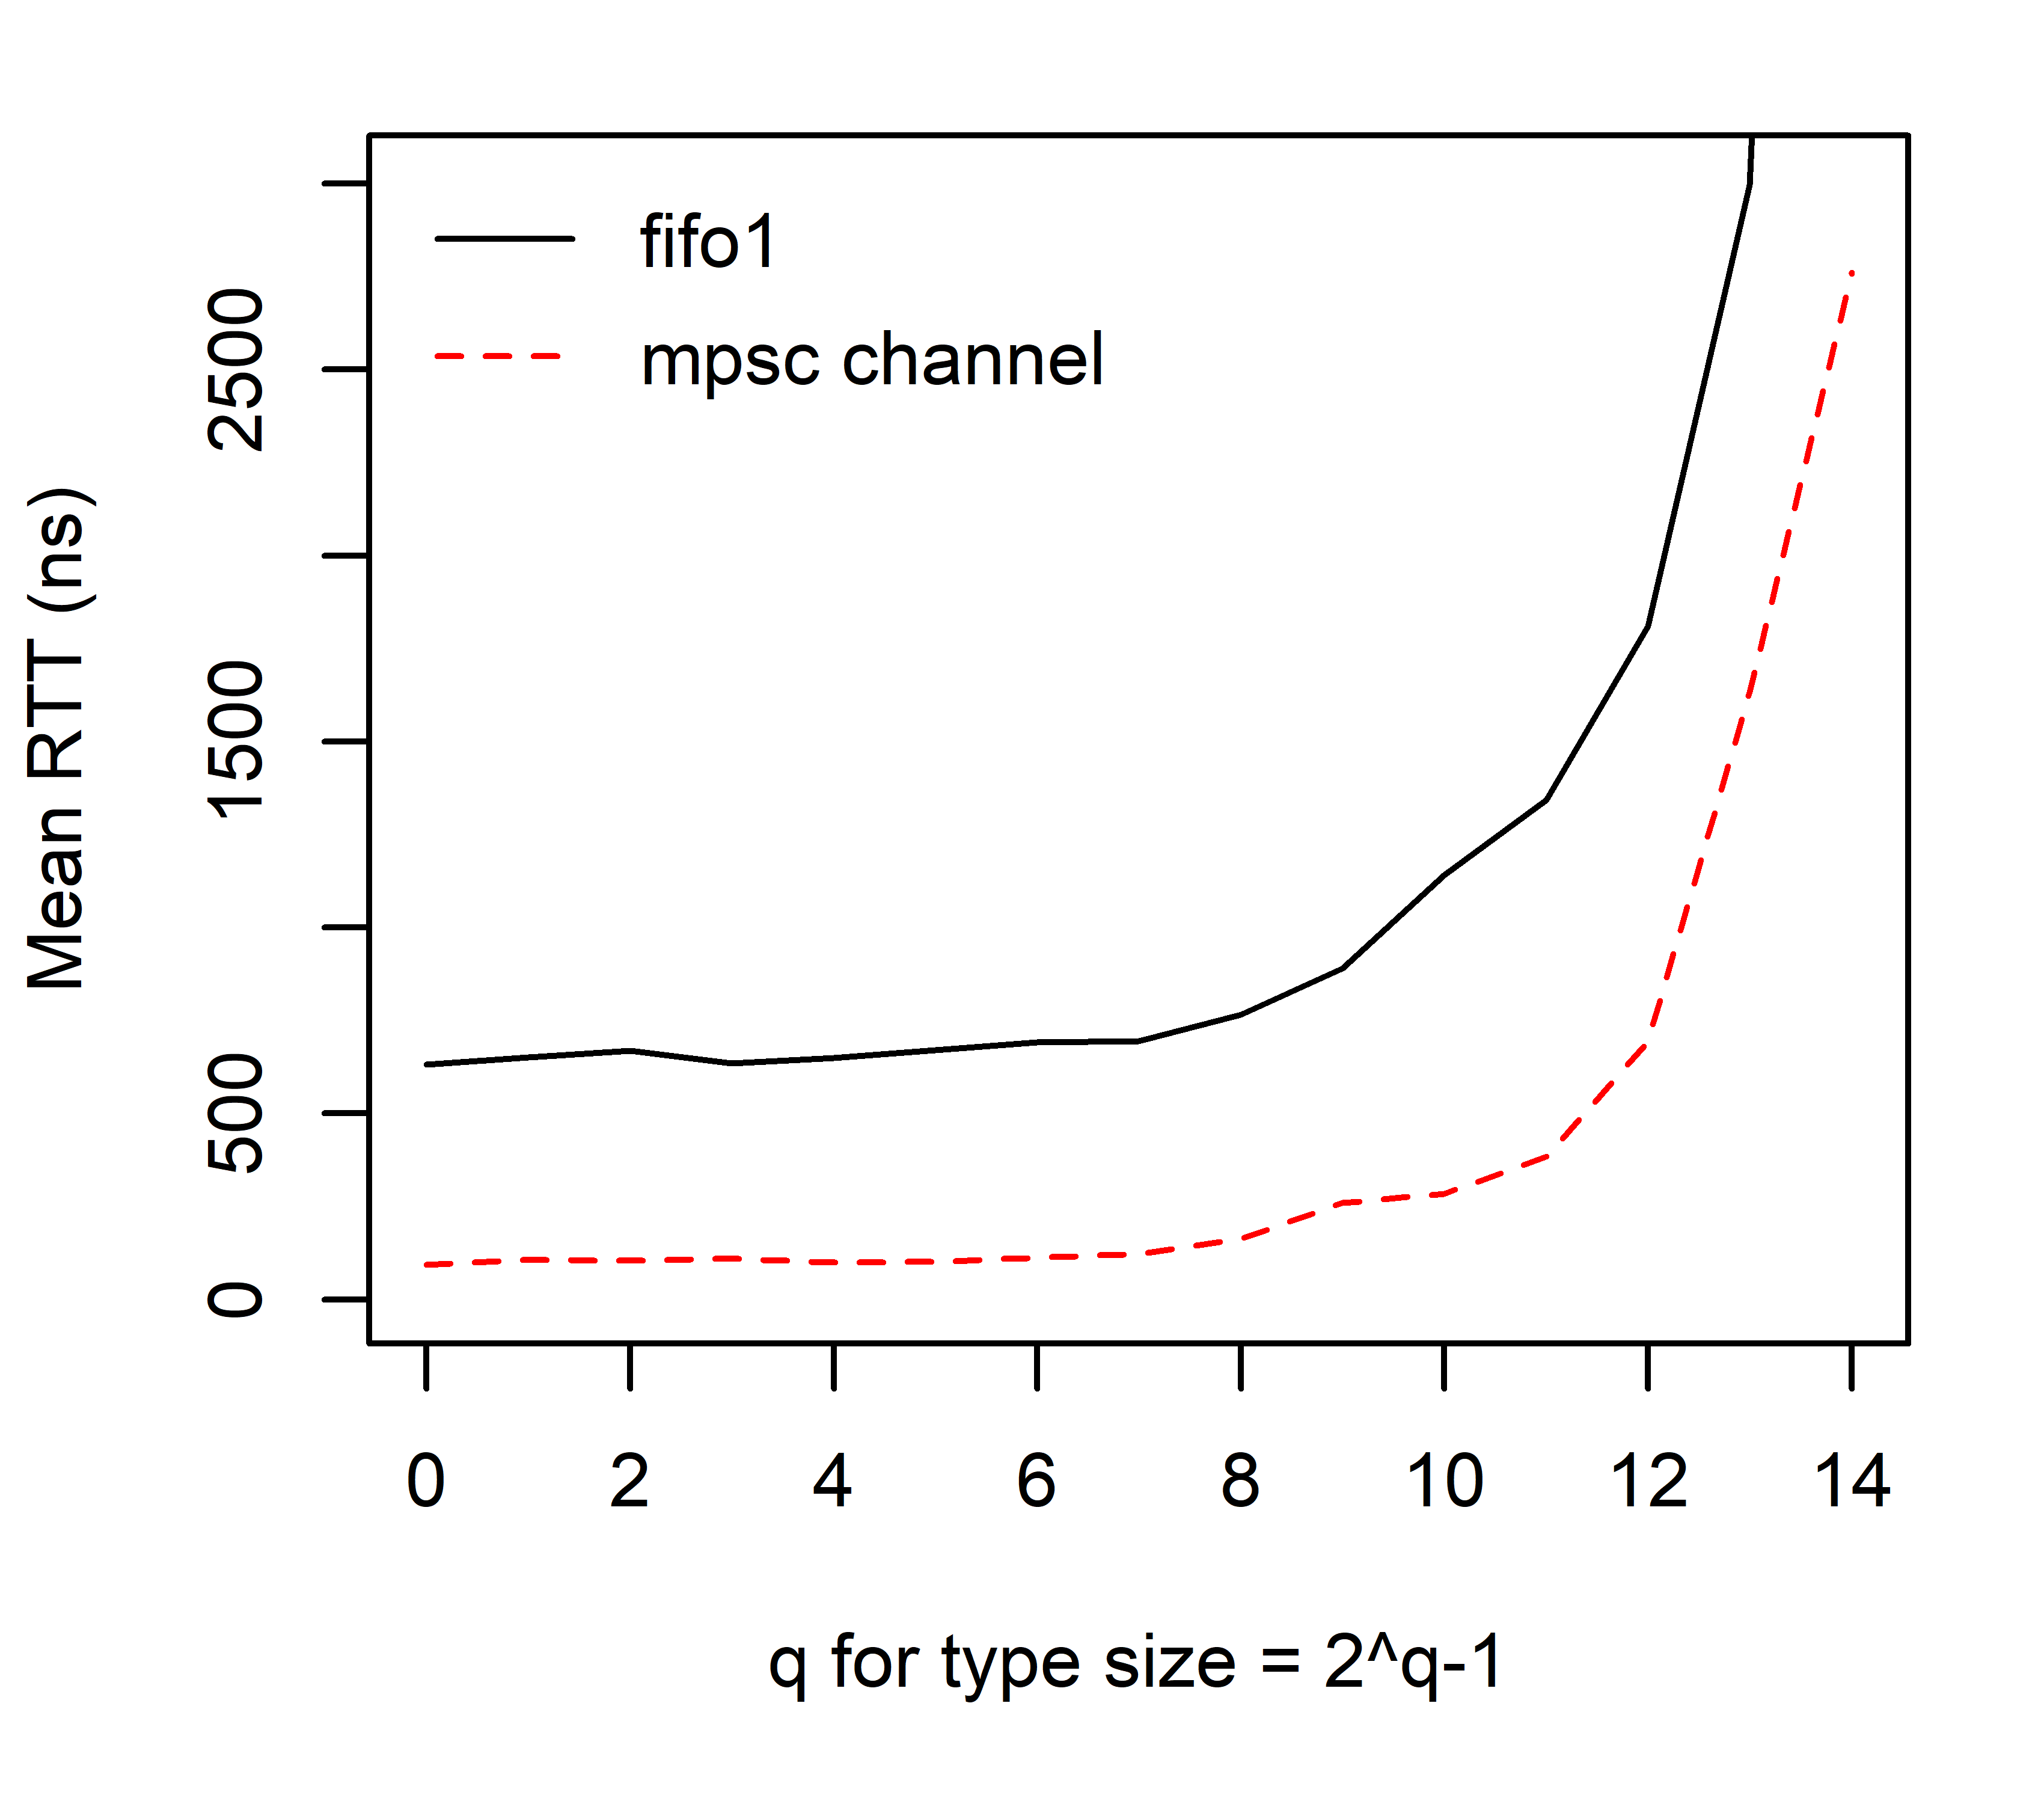
\includegraphics[width=\textwidth]{experiments/rtt_0.png}
			\caption{}
			\label{fig:exper_rtt_0}
		\end{subfigure}%
		\begin{subfigure}[b]{0.63\textwidth}
			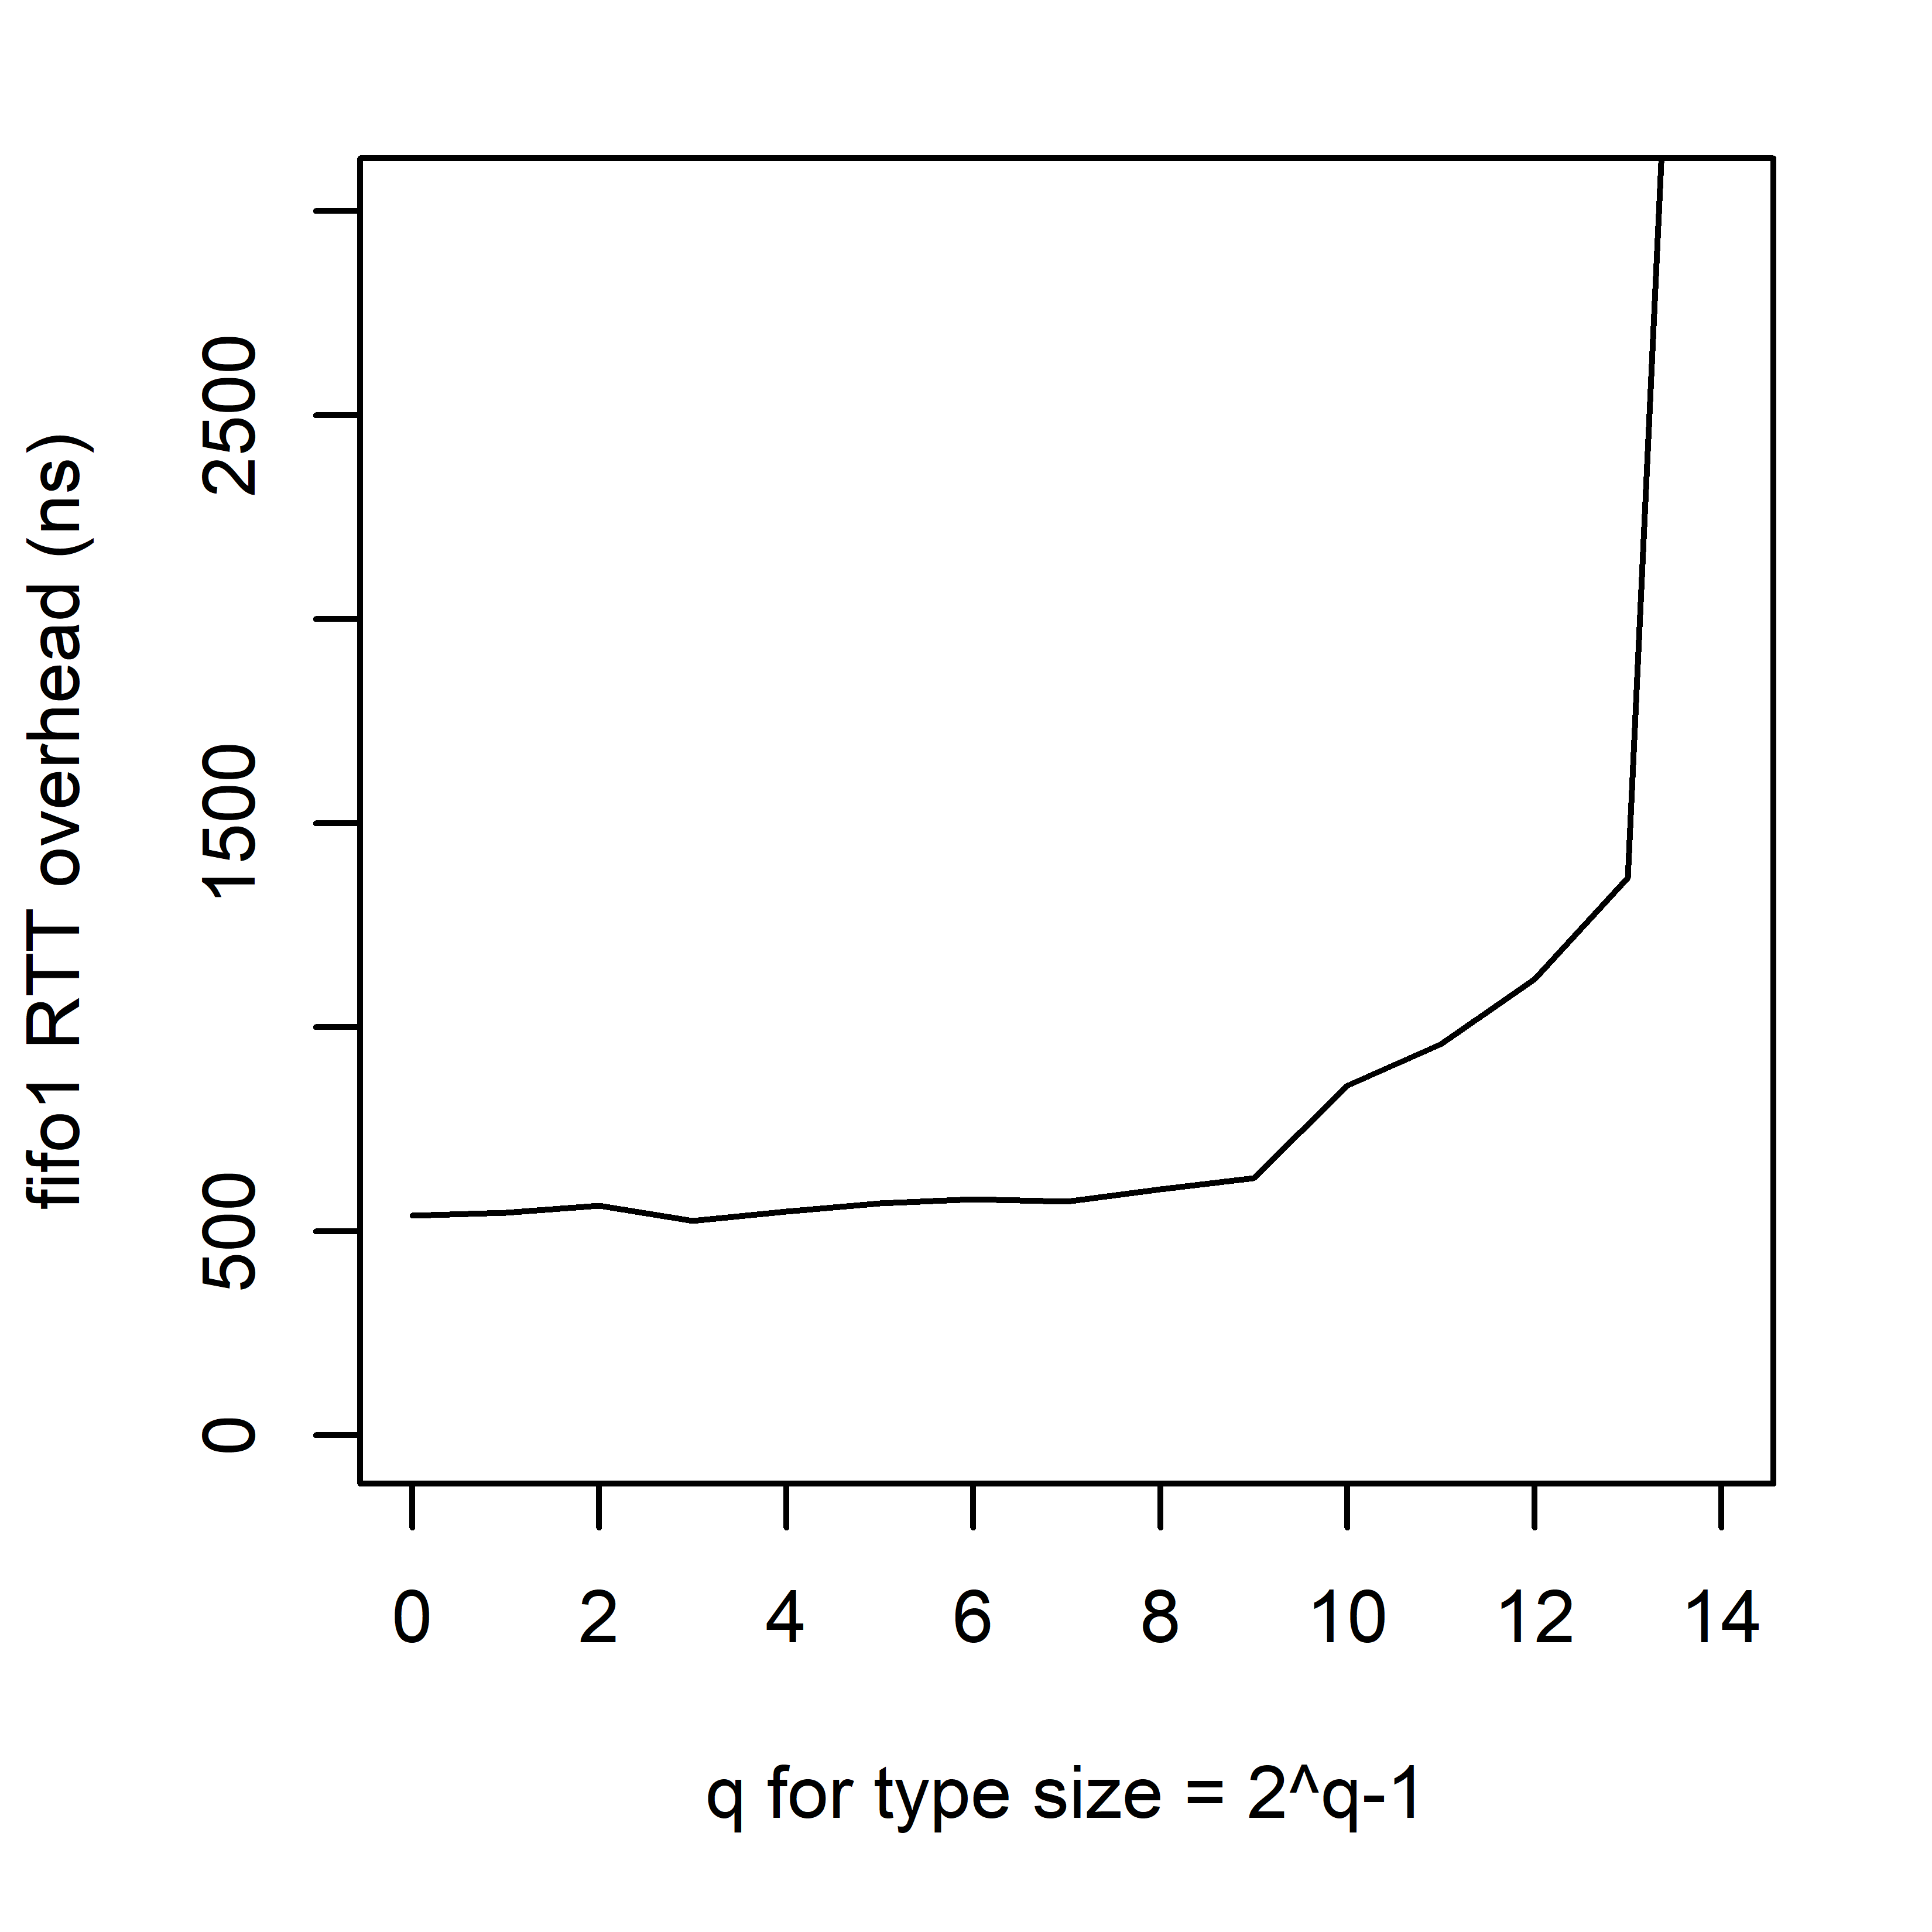
\includegraphics[width=\textwidth]{experiments/rtt_1.png}
			\caption{}
			\label{fig:exper_rtt_01}
		\end{subfigure}%
	}
	\caption[Performance of fifo1 connector vs.\ a standard channel type.]{Time from beginning of \code{put} to end of \code{get} in connector \textit{fifo1} compared to the time taken to send and received over an \code{mpsc} channel from the Rust standard library. Plots show the overhead in response to the size of the moved data. Figure~(b) shows the difference between the curves in Figure~(a), showing the overhead of Reo-rs more explicitly.}
	\label{fig:exper_rtt}
\end{figure}


These measurements show the range of times taken in response to changes in the data's size. The figure makes clear that compared to \code{mpsc}, Reo-rs experiences significant overhead in all cases. Some uniform overhead is to be expected, as \code{mpsc} is purpose-built and optimized for precisely this scenario. Reo-rs lacks the ability to optimize for this protocol to the same extent. For example, as explained in Section~\ref{sec:chosen_design}, all port-operations involve the acquisition of a shared protocol lock. Conceptually, Reo-rs has all the information it needs optimize for this protocol and particular and match the performance of \code{mpsc}. The generality of Reo-rs inhibits its ability to identify and specialize for these kinds of optimizations to the same extent as was done by hand for \code{mpsc}. A hand-optimized fifo1 channel could take advantage of the fact that the two ends of the channel need not share a lock at all. For this protocol, partitioning the coordinator such that each part only considers \textit{local} rules would be correct and cause less contention.

Figure~\ref{fig:exper_rtt_01} makes clear that Reo-rs is experiencing overhead that increases with the size of the moved value. At first glance, one can be forgiven for attributing this overhead to the presence of redundant movements of the data, which Section~\ref{sec:port_operations} explains can occur if llvm fails to optimize away the \textit{physical} movements from Rust's \textit{semantic} movements of values to new variable bindings. This turns out not to be the cause in this case. Rather, the overhead is caused by a more granular implementation detail; \code{mpsc} has a different method of moving its values. Listing~\ref{listing:mpsc_pop} gives a glimpse into how \code{mpsc} has some means to optimize data movements in the case of an x86-64 processor by `in-lining' it, spelling it out into a sequence of smaller movements hundreds of lines long. In this manner, \code{mpsc} is optimized to avoid the overhead of system calls.

\begin{listing}[h!]
	\centering
	\inputminted{text}{mpsc_pop.txt}
	\caption[x86-64 assembly of a standard Rust channel, showing in-lining.]{Snippet out of the x86-64 assembly generated by receiving a large datum through \code{recv} from a simple channel from the Rust standard library. It unrolls the movement of the entire object into a large sequence of smaller operations rather than invoking a system call.}
	\label{listing:mpsc_pop}
\end{listing}

\section{Overhead Examined}

\subsection{Port-Operation Parallelism}

For connectors as simple as \textit{fifo1}, overhead is overhead. However, we are particularly interested in understanding how this overhead is partitioned; as connectors become more complex, different parts of this overhead impact \textit{parallelism} in different ways. Section~\ref{sec:protocol_runtime} explains the nature of the \textit{coordinator} role, and how its operations are performed holding the lock for the \code{Proto} instance which connects ports as their common communication medium. Table~\ref{tab:active_time} shows measurements for an experiment that attempts to understand which proportion of our overhead is incurred \textit{inside} the critical region, ie.\ by the coordinator. In the case of this experiment, our protocol has rules for movement which can be rendered as a \textit{bipartite graph}, allowing data flow from any putter in $\{P0, P1, P2\}$ to any getter in $\{G0, G1, G2\}$. As explained in Section~\ref{sec:data_exchange}, movements such as these do not buffer the data elements inside the protocol; getters take values from putters directly. As a consequence, putters are both the first and last to parttake in any of our rule firings' data movements. The table shows the mean duration for which each putter was involved in such a firing. Along with the total duration of the run, we are able to compute to which extent these putters were able to work in parallel. We distinguish between four cases, corresponding to rows in Table~\ref{tab:active_time}. The first three cases do not involve the \code{clone} operation, and are observed to have insignificant differences for all measurements. For this experiment, with modestly-sized values, we conclude that there is no large difference in performance between these three cases:
\begin{enumerate}
	\item [\textbf{move}] Values are moved from putter to getter synchonously.
	\item [\textbf{copy}] Putters retain their values, and getters replicate them with a bit-wise copy that does not mutate the original.
	\item [\textbf{signal}] Getters do not return any data. They return after releasing putters.
\end{enumerate}

The final \textbf{clone} case attempts to observe the effects of intentionally delaying getters outside of the lock by necessitating the use of an explicit \code{clone} operation whose duration is artificially lengthened\footnote{\code{sleep} calls were out of the question, as its variability is overwhelming at this scale. Instead, \code{clone} perform thousands of chaotic integer computations on the replica before returning it. This is intentionally obtuse such that the Rust compiler is unable to identify a trivializing optimization.}. For these runs, putters retained their original values, but the datum was not marked with the \code{Copy} trait. In all cases, we observed that even at this coarse granularity, there was significant parallelism. For the majority of the time, new rules were able to fire whilst interactions were being completed outside of the critical region. The final case in particular was within a small rounding error of perfect parallelism.

\begin{table}[]
	\begin{tabular}{l|lll|ll}
		& \multicolumn{3}{l|}{mean active time} & \multirow{2}{*}{\begin{tabular}[c]{@{}l@{}}run\\ duration\end{tabular}} & \multirow{2}{*}{\begin{tabular}[c]{@{}l@{}}mean\\ parallelism\end{tabular}} \\
		& p0 & p1 & p2 &  &  \\ \hline
		move & 2.037µs, & 2.031µs, & 2.017µs & 214.991ms & 2.83 \\
		copy & 1.744µs, & 1.852µs, & 1.844µs & 197.676ms & 2.75 \\
		signal & 1.962µs, & 1.956µs, & 1.937µs & 207.181ms & 2.83 \\
		\hline
		clone & 94.021µs, & 94.082µs, & 94.058µs & 9420.148ms & 2.995 
	\end{tabular}
	\caption[Parallelism between getters in runs of the SISO connector.]{Runs of 3 putters greedily sending their data directly to any of 3 getters, 100000 times. This test was performed with 4~variants, differing on the properties of the data and whether the putter retained the original. The last column is derived, showing to what extent these putters were able to work in parallel.}
	\label{tab:active_time}
\end{table}

\subsection{Overhead Inside the Critical Region}
The previous section, we saw an experiment with data moving between putters and getters. These runtimes included the putter's time spent not only on the movement itself, but also on the time spent in the role of \textit{coordinator}. Here, we examine the work that pertains to this role and how changes to the definition of rules influence overhead. Figure~\ref{fig:check_time} shows the overhead incurred by a coordinator that traverses \textit{unsatisfied} rules before finding one to fire. It is apparent that in all cases, the overhead scales linearly, as expected. The time taken to evaluate the satisfaction of a rule varies greatly dependent on its definition; the evaluation of a rule involves many different operations mirroring the intricacies of the \textit{imperative form} it models, described in Chapter~\ref{sec:imperative_form}. To represent the possibility space, the figure shows measurements for a simple protocol which encounters replicas of one unsatisfied rule repeatedly, where its nature comes in four distinct variants:
\begin{enumerate}
	\item [\textbf{guard}] A rule where some port is not ready. This is detected almost immediately by cheap \textit{bit vector} operations, as explained in Section~\ref{sec:minimizing_the_bottleneck}. Evaluation takes 8.76ns.
	
	\item [\textbf{false}] A rule whose first instruction checks the predicate \textit{false}. Evaluation takes 18.91ns.
	\item [\textbf{ands}] A rule whose first instruction is a tree-like formula structure of twenty-five conjunctions, only the last of which is \textit{false}. Evaluation takes 180.72ns.
	\item [\textbf{alloc}] A rule whose first instruction allocates a fresh boolean-type resource with value \textit{false}. The second instruction checks that this temporary value is true. Upon failure, the allocation must be rolled back, discarding the temporary value. Evaluation takes 316.51ns.
\end{enumerate}


\begin{figure}
	\centering
	\makebox[\textwidth][c]{
		\begin{subfigure}[b]{0.63\textwidth}
			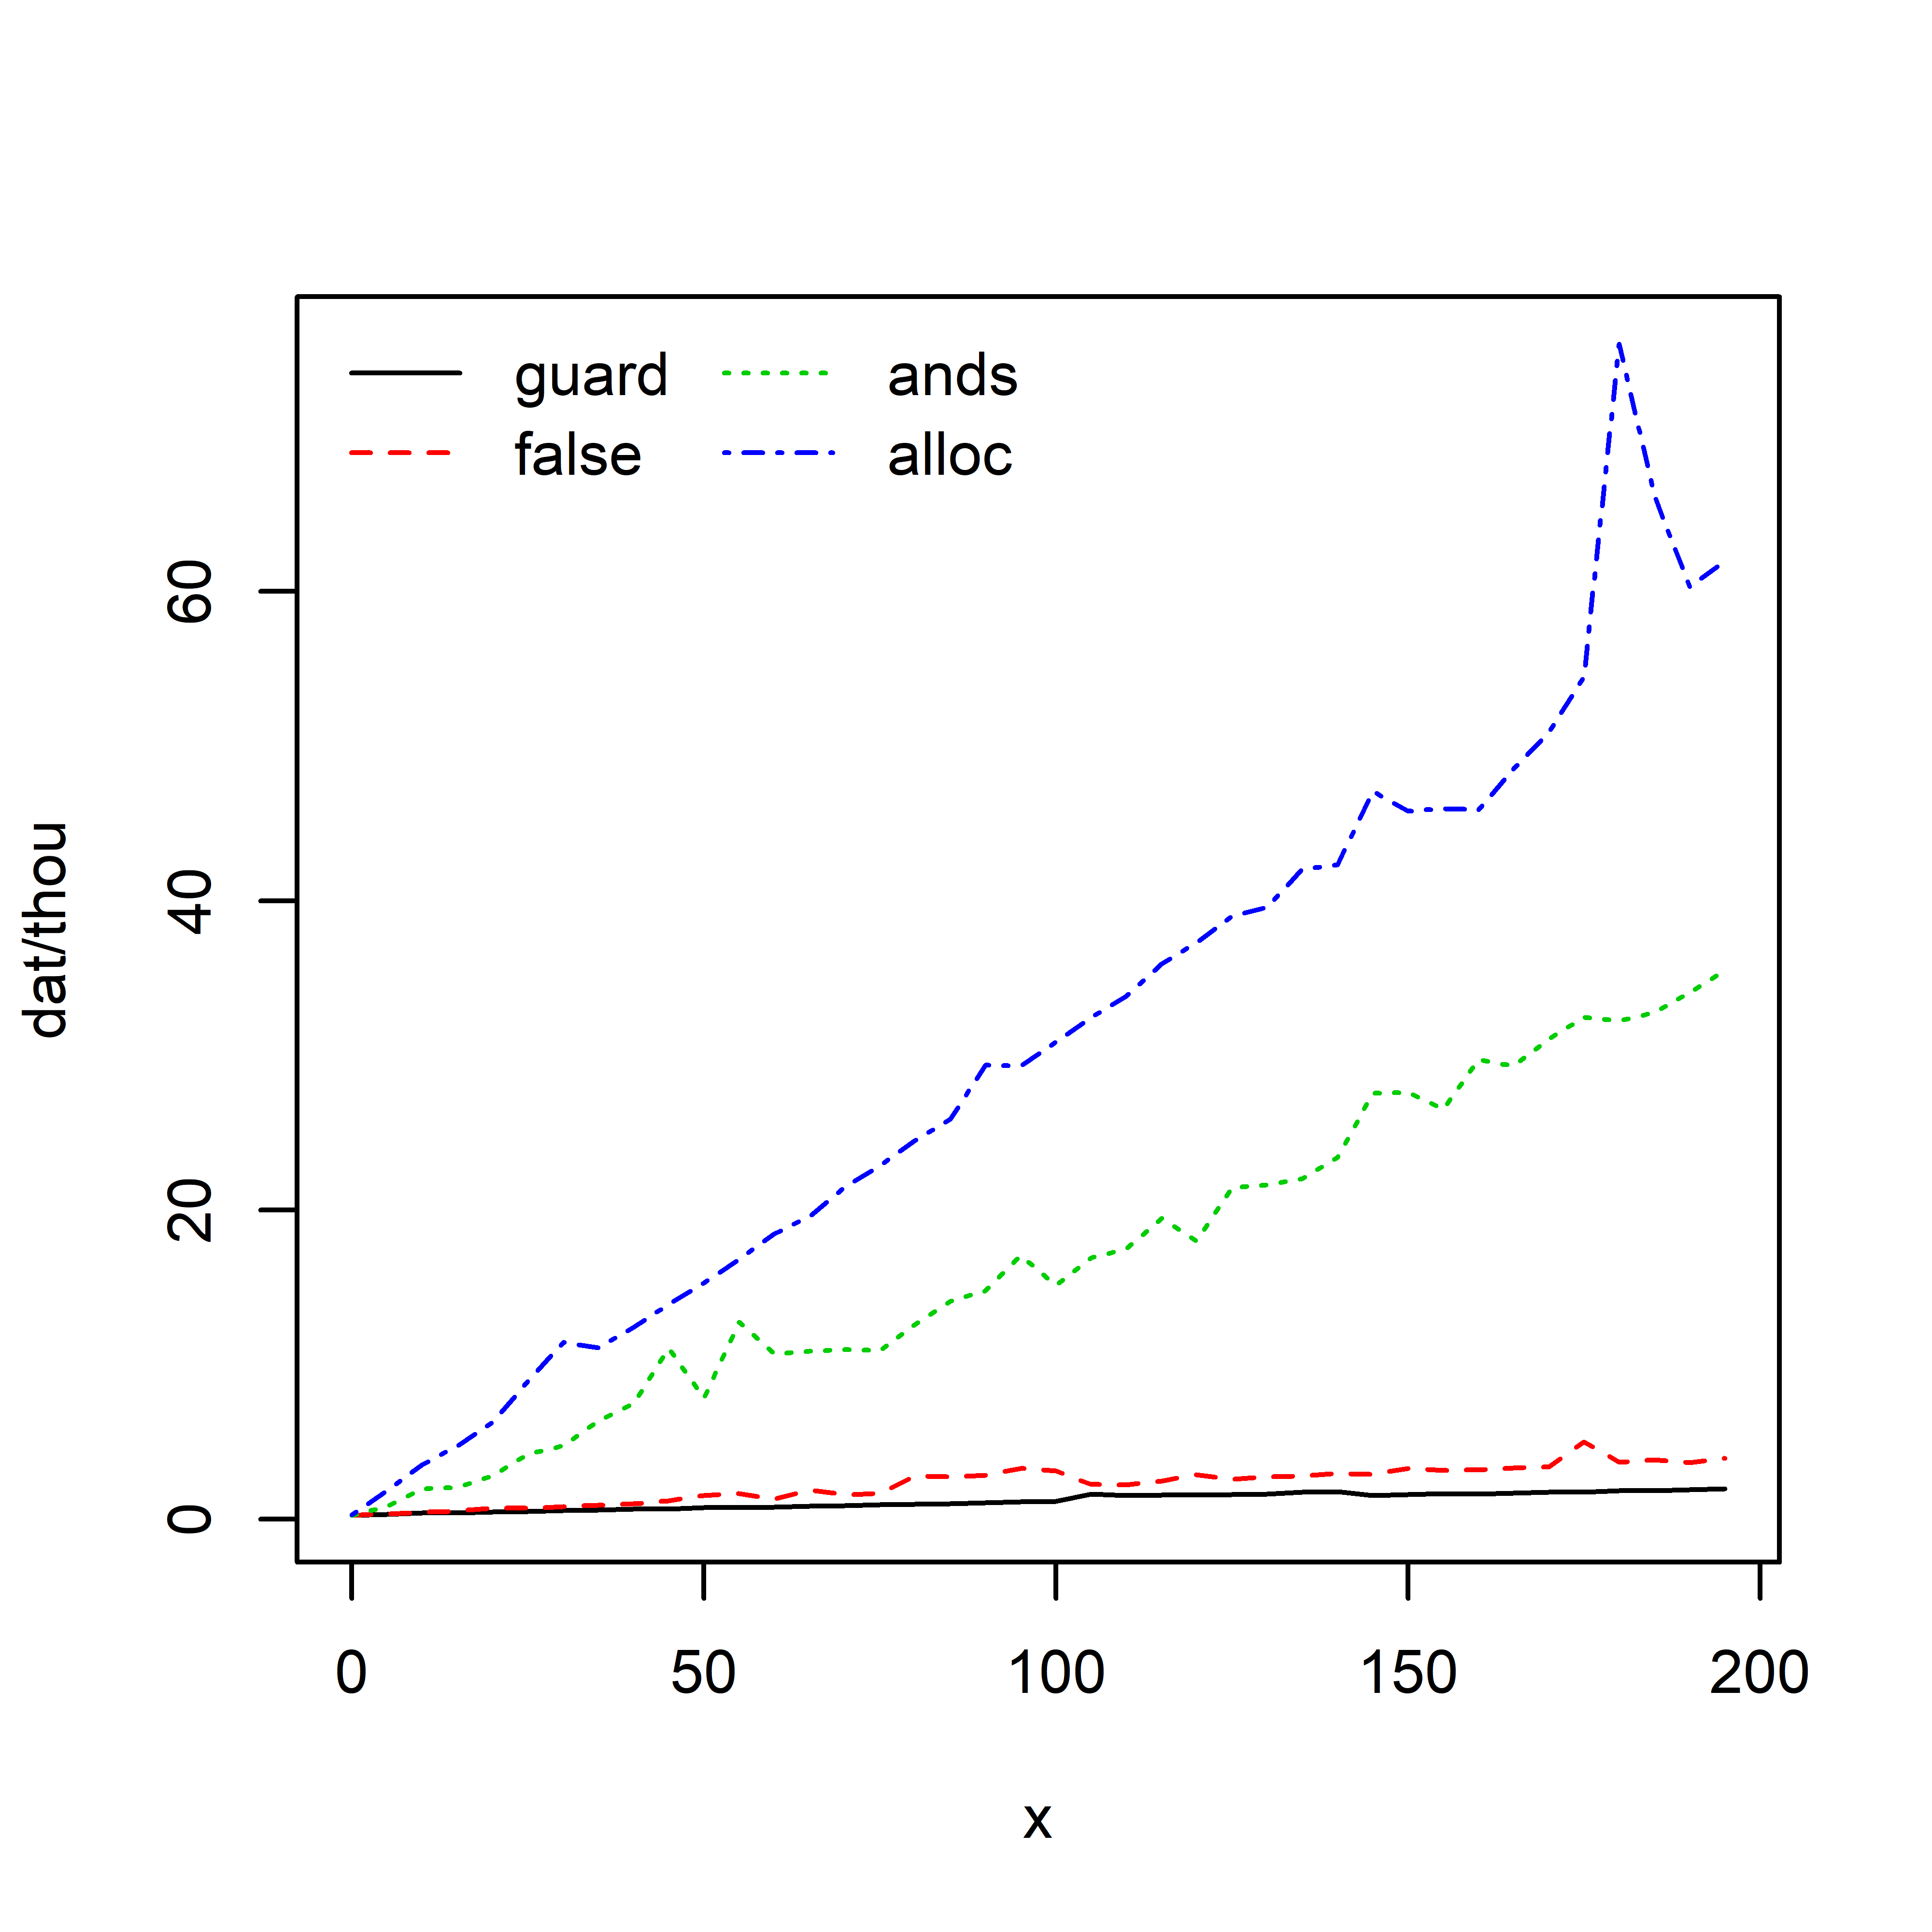
\includegraphics[width=\textwidth]{experiments/check_time_0.png}
			\caption{}
			\label{fig:check_time_0}
		\end{subfigure}%
		\begin{subfigure}[b]{0.63\textwidth}
			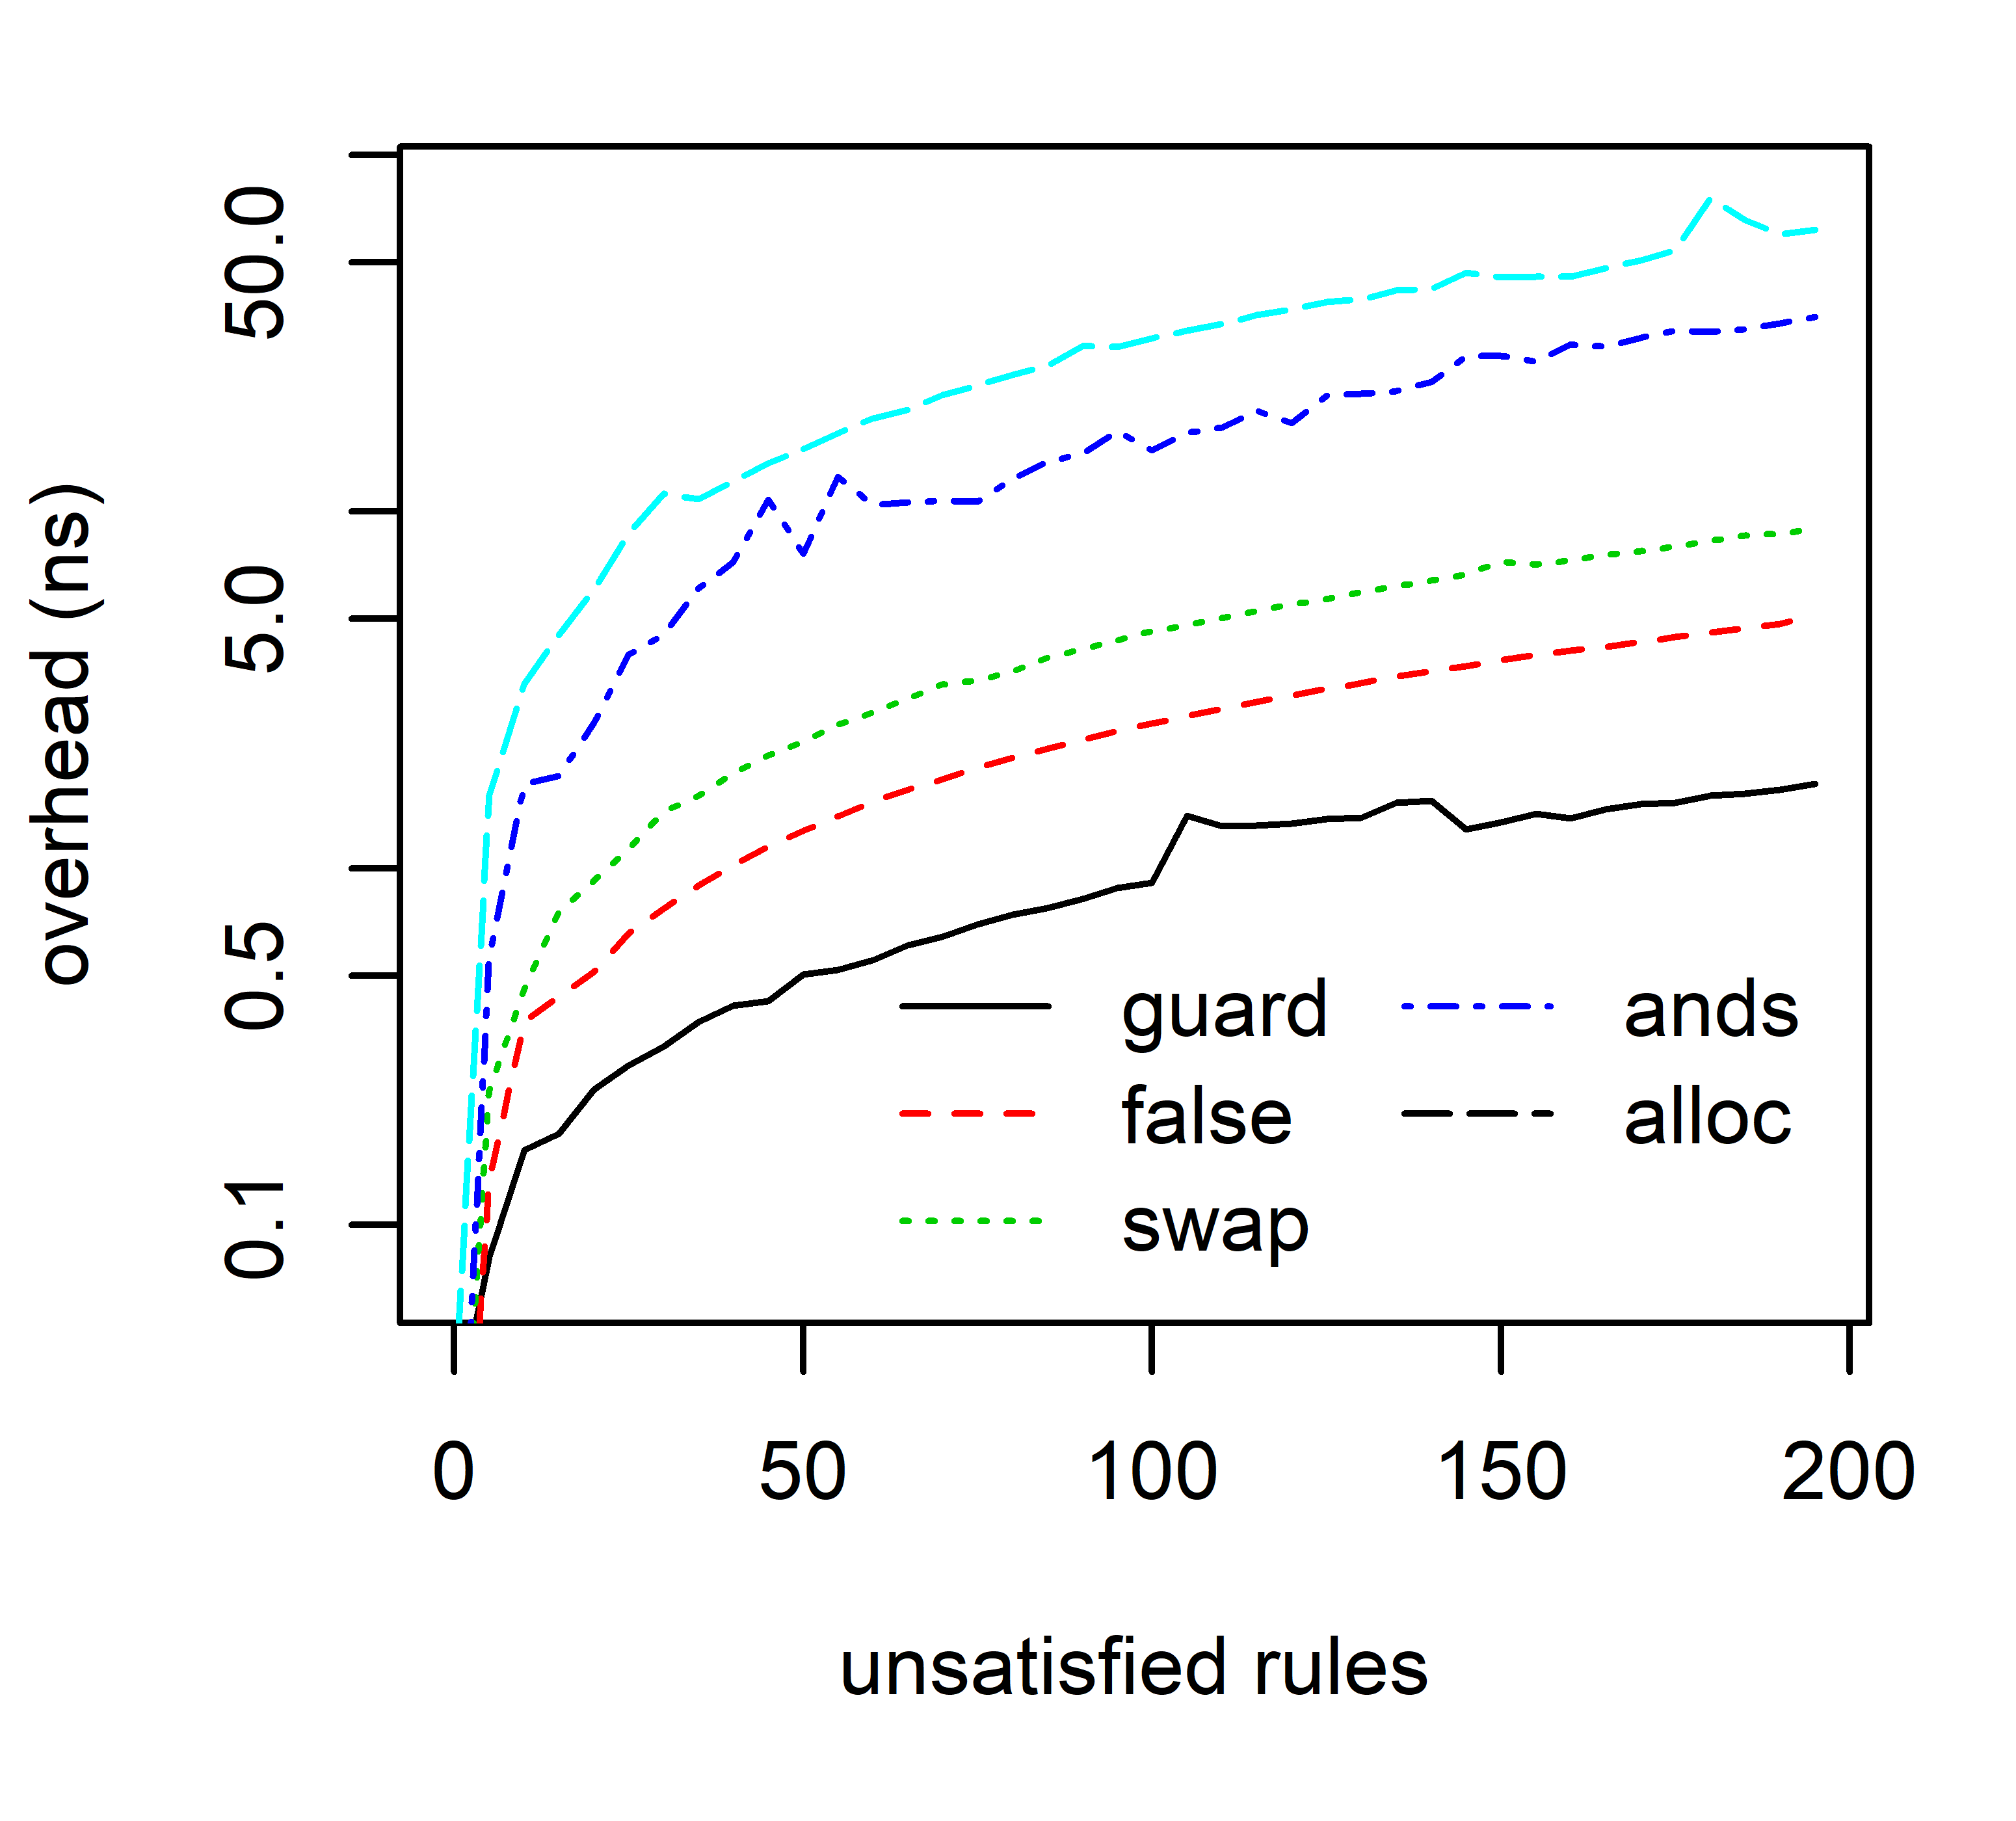
\includegraphics[width=\textwidth]{experiments/check_time_1.png}
			\caption{}
			\label{fig:check_time_2}
		\end{subfigure}%
	}
	\caption[Overhead of evaluating unsatisfied rules.]{Overhead as a result of evaluating a sequence of identical unsatisfied rules before firing something. Experiment is repeated for four variants of unsatisfied rules varying in the complexity of the operations they before before being deemed unsatisfied. The two sub-figures show the same information, with (b) representing it with a logarithmic y-axis to accentuate the small-scale differences.}
	\label{fig:check_time}
\end{figure}

These results meet our expectations. Rules can be arbitrarily complex, and perform an arbitrary amount of work before concluding that they are not satisfied, and will not fire. Even for this small set of relatively simple examples, we are able to see orders of magnitude in difference between the best case (in which the rule is skipped as early as possible by evaluating a bit-vector), to the worst case (involving several complex instructions). Fortunately, realistic Reo connectors will be defined almost entirely by rules that are either skipped as a result of evaluating these bit-vectors, or not at all. Even more expensive guards can expect to incur overhead in the order of nanoseconds as long as they involve no more than a handful of reasonable instructions. 

\begin{figure}
	\centering
	\makebox[\textwidth][c]{
		\begin{subfigure}[b]{0.63\textwidth}
			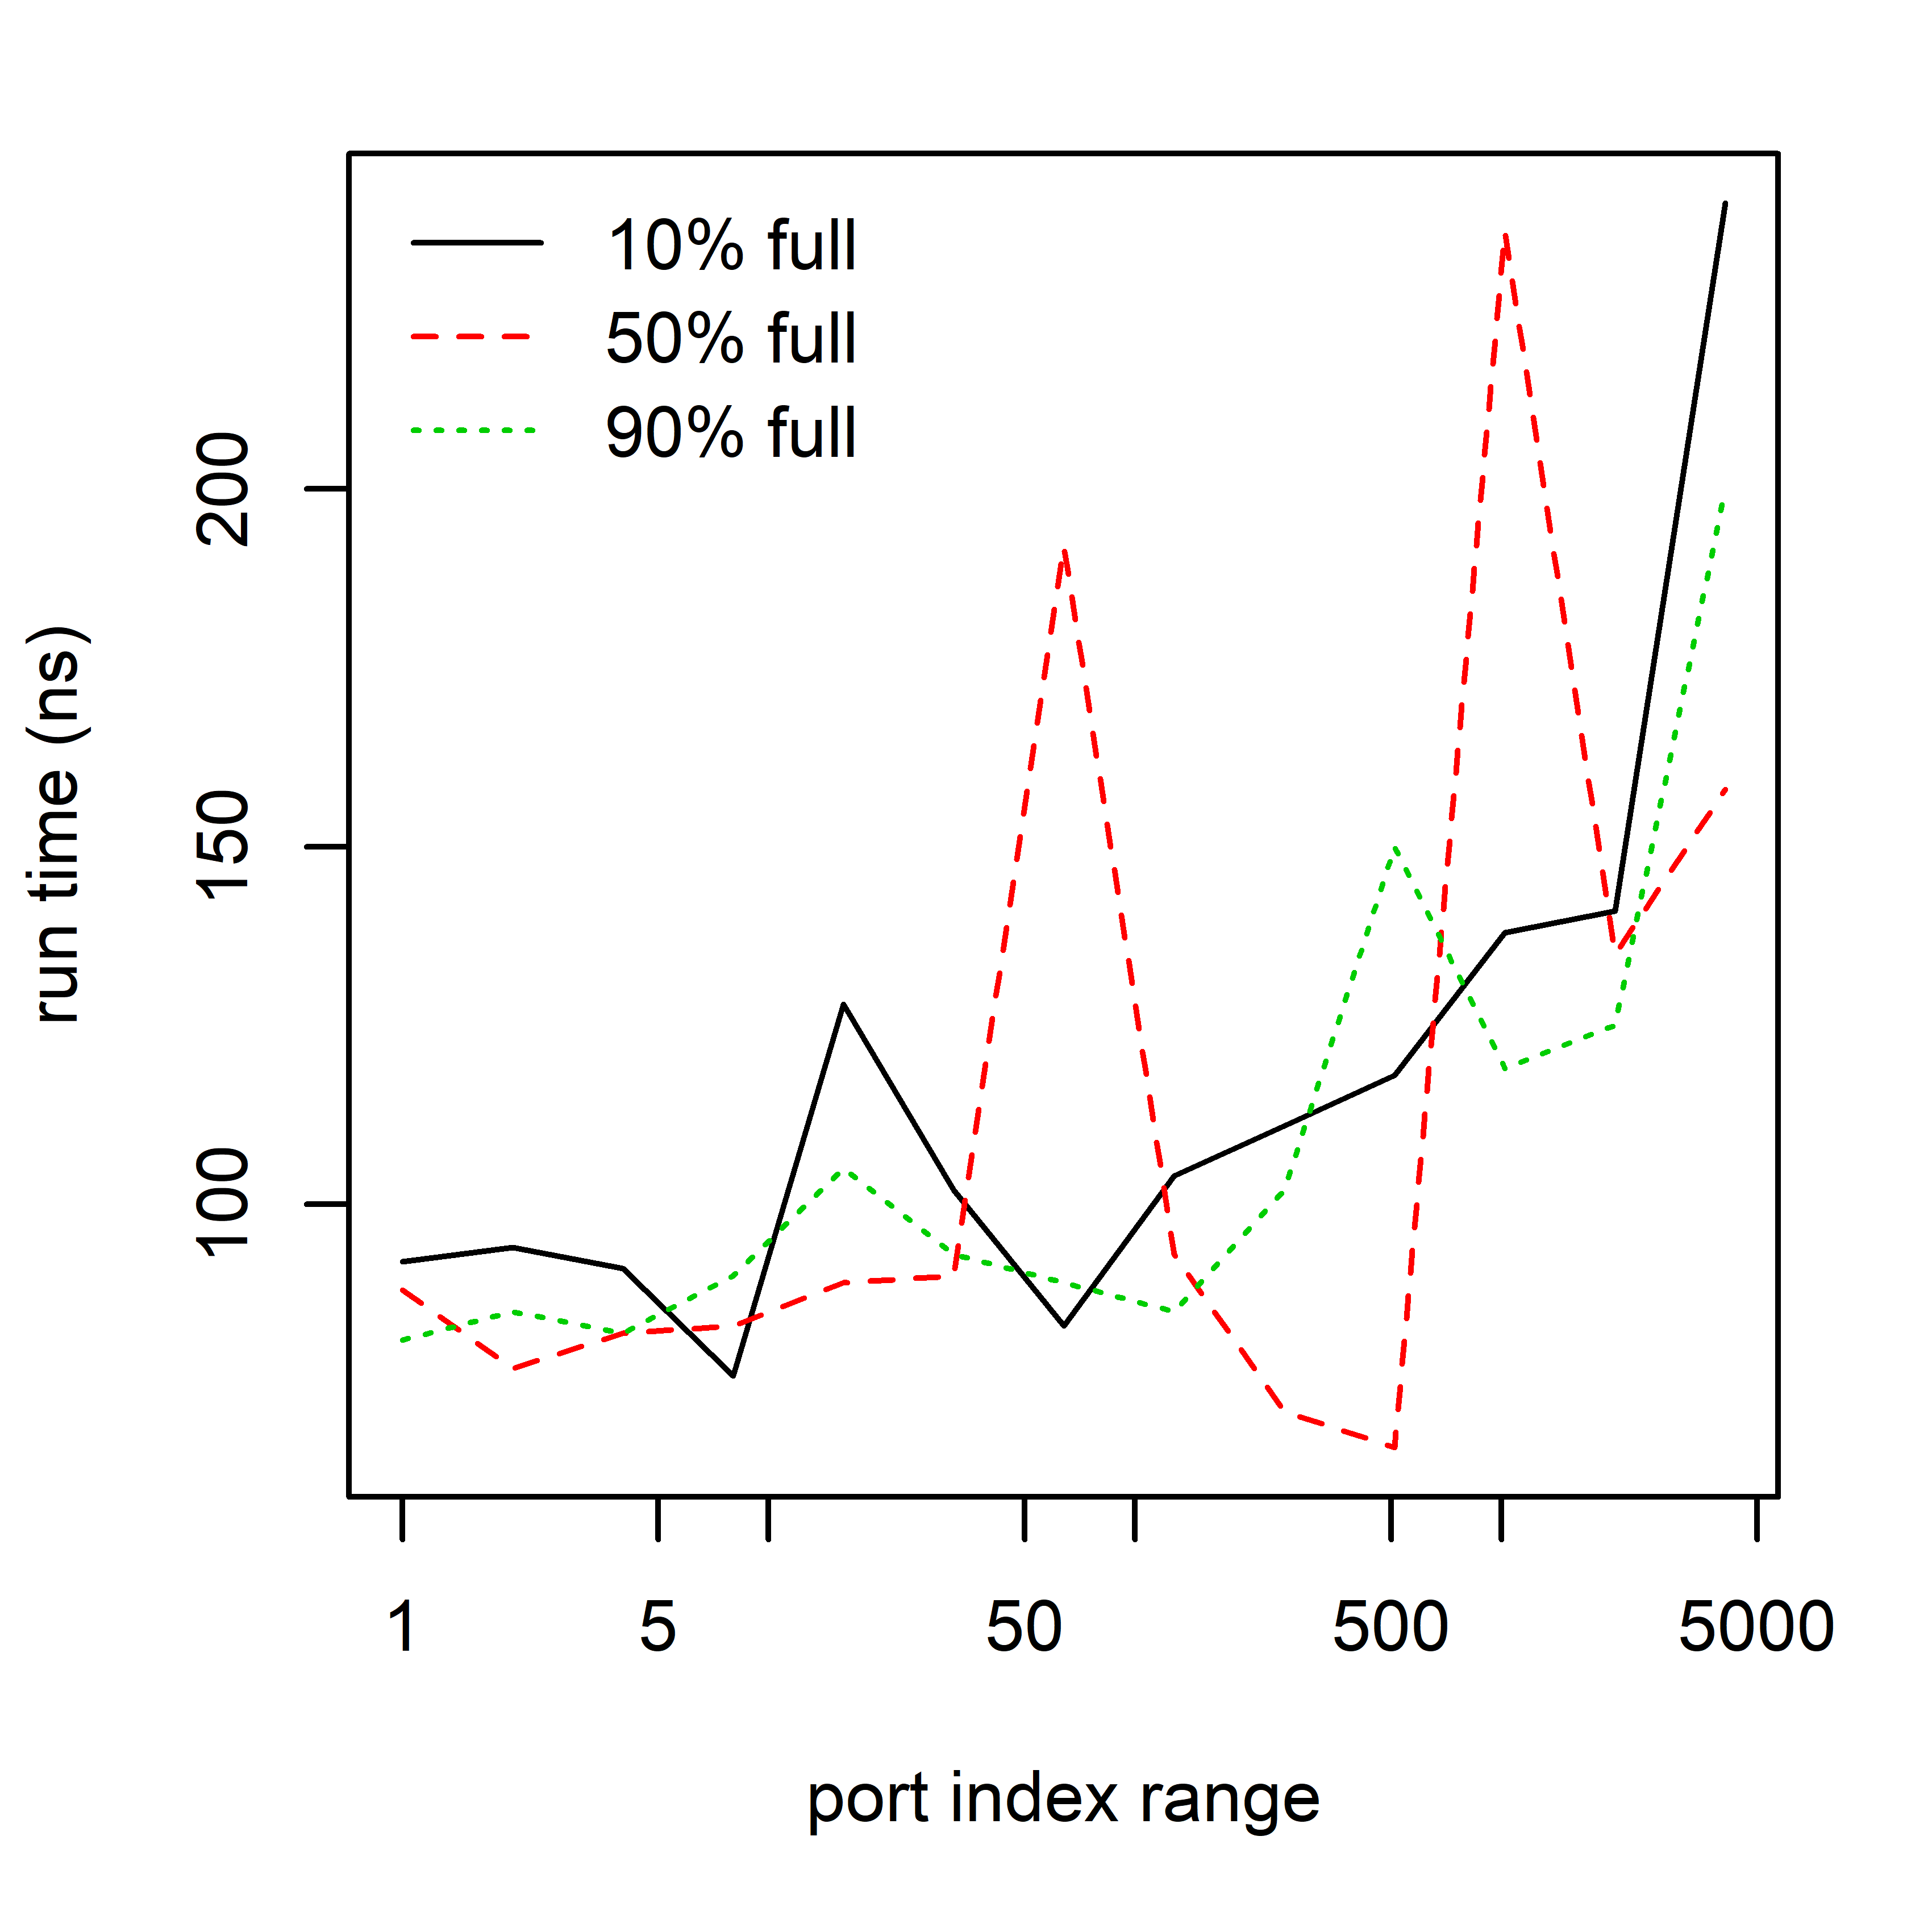
\includegraphics[width=\textwidth]{experiments/bits_0.png}
			\caption{}
			\label{fig:bits_0}
		\end{subfigure}%
		\begin{subfigure}[b]{0.63\textwidth}
			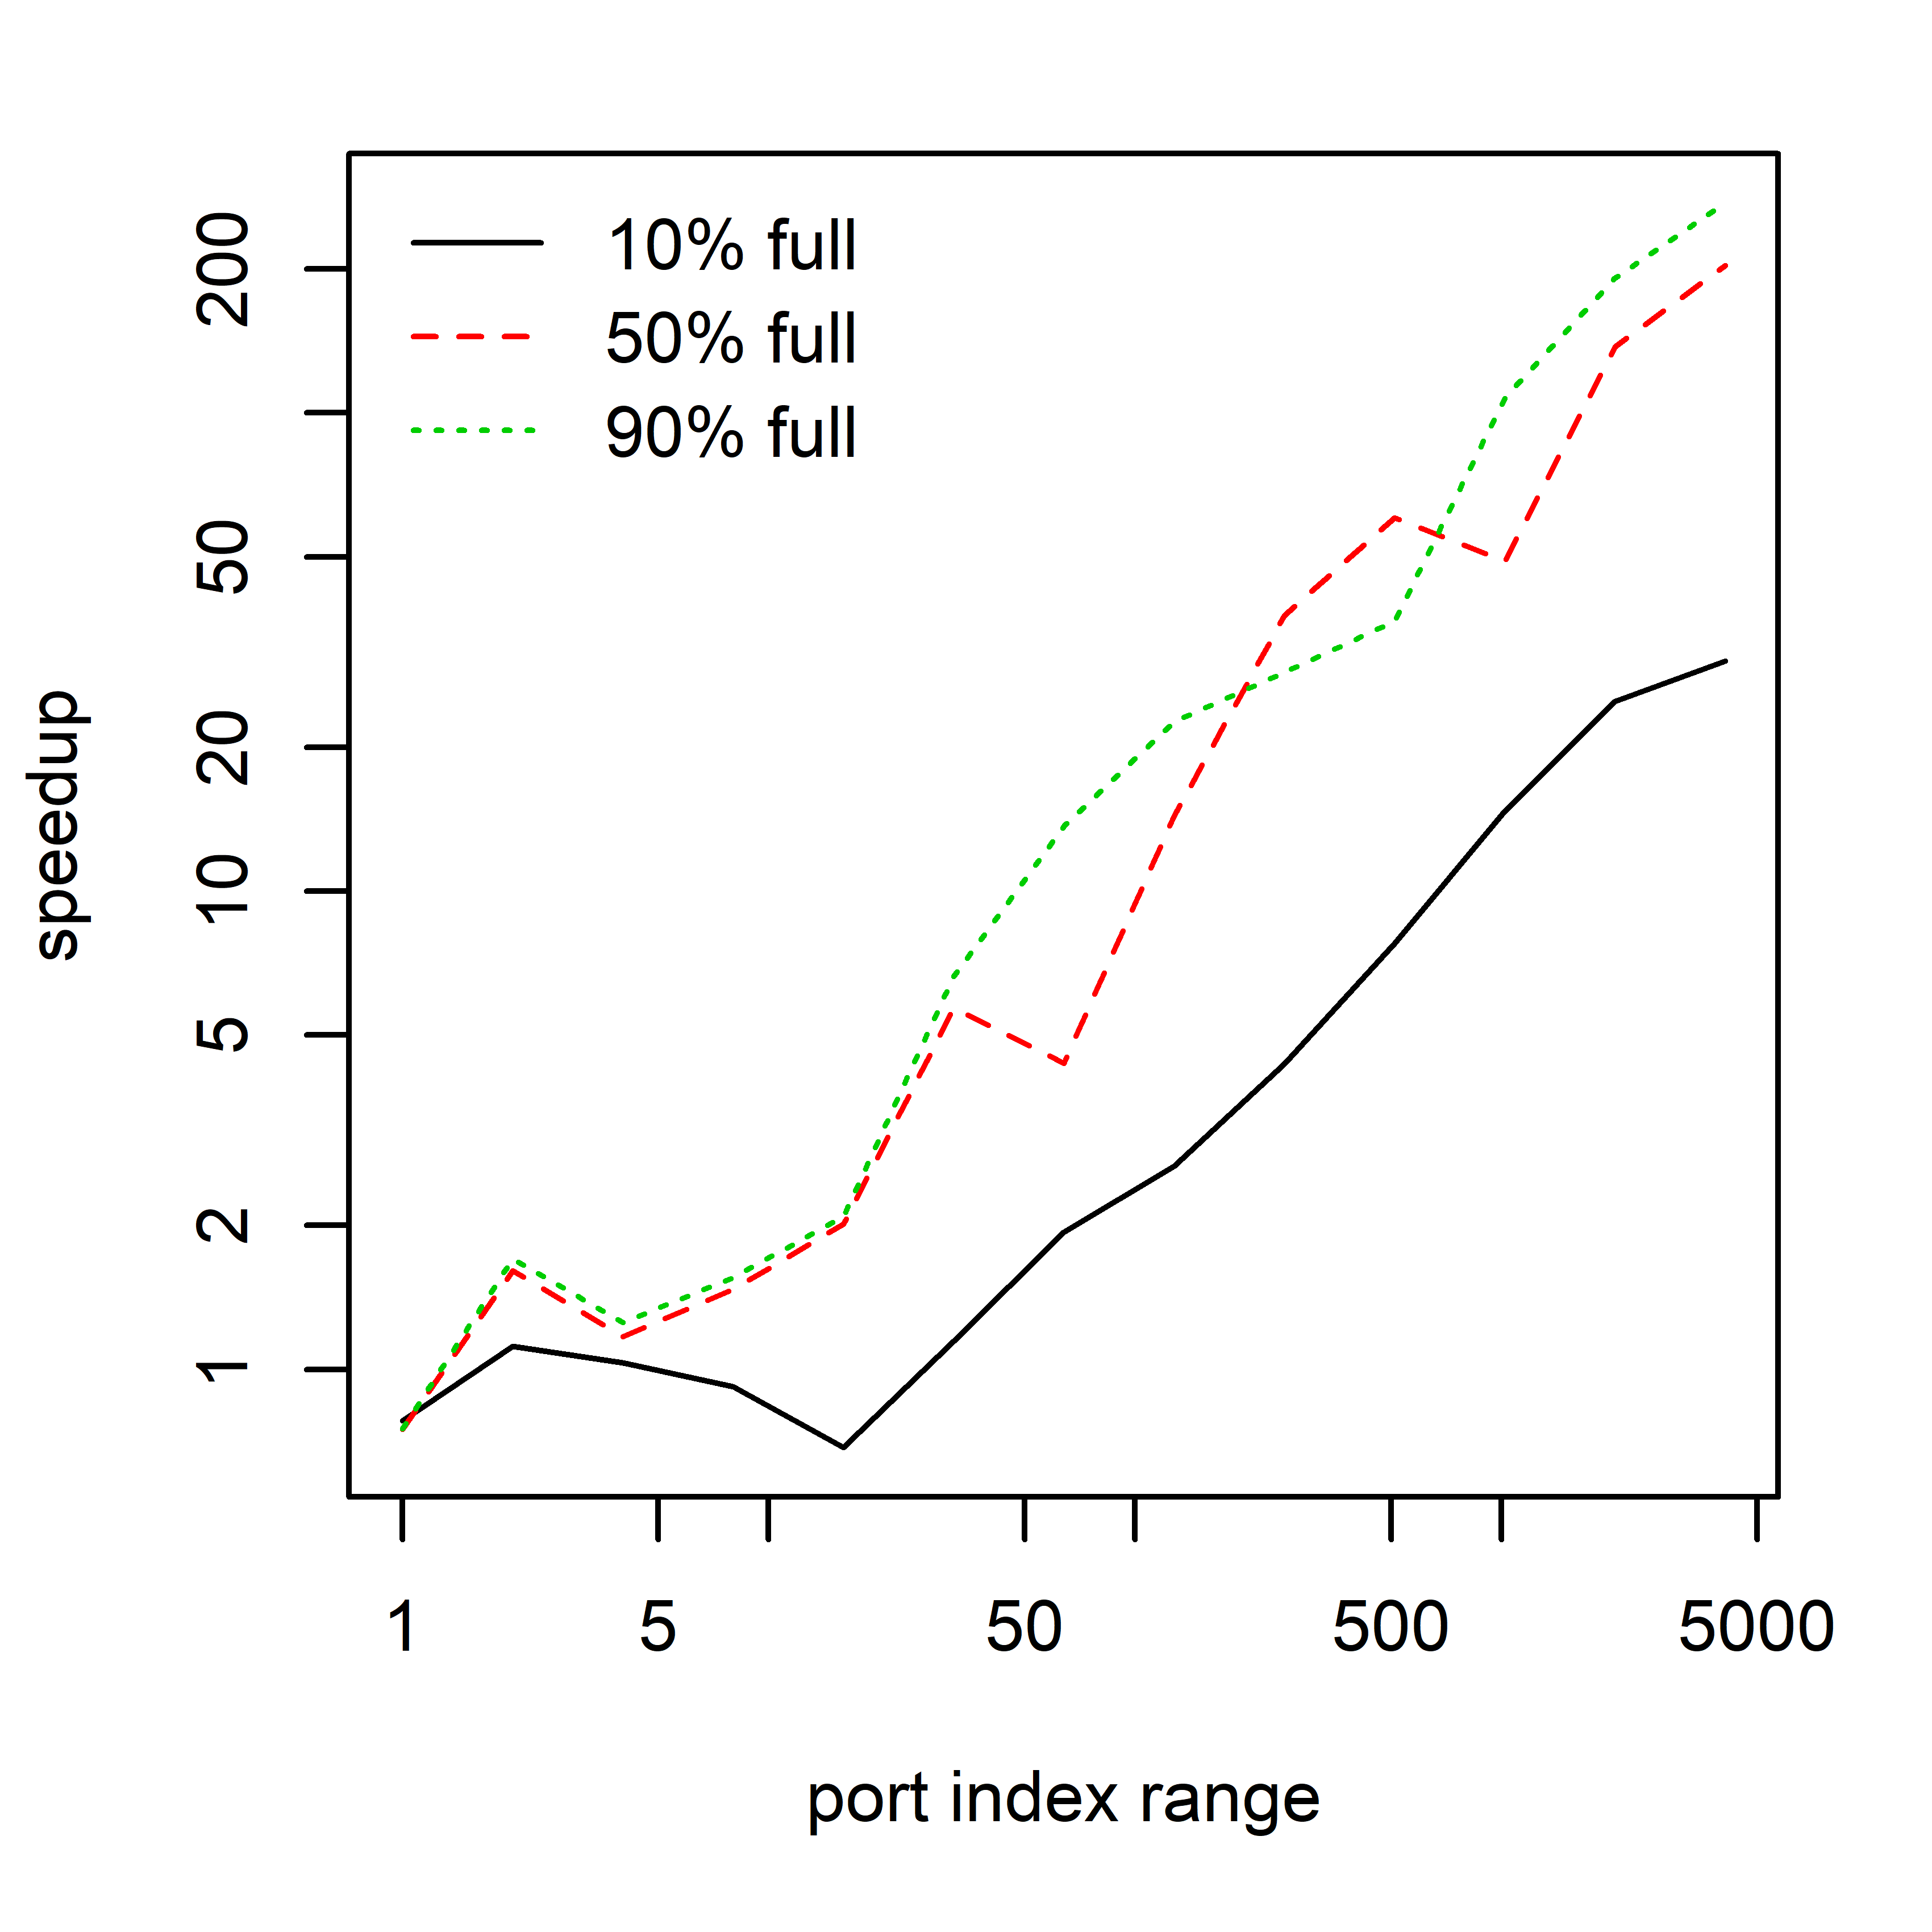
\includegraphics[width=\textwidth]{experiments/bits_1.png}
			\caption{}
			\label{fig:bits_1}
		\end{subfigure}%
	}
	\caption[Bit vector speedup over hashset.]{Run time of the \code{is\_subset} operation for bit vectors and canonical hash sets. This operation is used very frequently by the coordinator to determine whether a rule is satisfied. Figures show (a) run times for the bit vector in response to a changing maximal element, ie.\ number of ports, and (b) the speedup of the bit vector in comparison to the hash set. Note the logarithmic axes.}
	\label{fig:bits}
\end{figure}



The efficiency of the bit vector \textit{subset} operation is key to the speed of the coordinator. This is the first first three things evaluated for each and every rule, checking whether all involved ports are ready, and if all the relevant memory cells are full or empty. The bit-set capitalizes on how unusually often we need this operation. Figure~\ref{fig:bits} shows how bit vectors are very efficient at checking whether one is a subset of another. Here we see the time taken to evaluate the \textit{positive} case, representing the best-case scenario for our speedup. It is guaranteed to occur at least three times every time a rule fires. Figure~\ref{fig:bits_0} shows how low the cost of the operation stays, even when there are very many ports involved. Figure~\ref{fig:bits_1} shows how significant the speedup over the subset operation of canonical \code{HashSet} type. Admittedly, the majority of realistic Reo circuits are on the low-end with respect to number of ports; if nothing else, this is a result to encourage the development of more complex connectors. Observe that the cost of the operation is agnostic to the \textit{fullness} in the case of the bit-vector. This is not so for the hash set, for which a fuller hash set makes for a more expensive operation. 



\subsection{Overhead Outside the Critical Region}
After data exchanges are initiated by the coordinator, the protocol's lock is released. Time spent exchanging can therefore only impact the threads that play a part directly. Figure~\ref{fig:simo_copy} shows measurements of the \textit{siso} protocol, which synchronously distributes a putter's datum to a set of getters. First, we concentrate on the case where this datum implements the \code{Copy} trait, communicating to Reo-rs that it is safe to replicate elements of the ports' data type with bit-wise shallow copies. The experiment shows the mean time to finish one such interaction, varying in response to the size of the datum, and repeated for a different number of getters. As expected, runs with more getters took longer to complete, as the putter cannot return until everyone else is finished. The cost of the copy operations can also be seen to grow approximately linearly. Figure~\ref{fig:simo_copy_1} shows the runs normalized to that of the case with a single getter; here we observe that as the data gets larger, the overhead of the additional getters decreases in proportion to that of the single getter. The measurements for four and five getters are unexpectedly high compared to the rest. We are not able to fully explain this, and imagine it has something to do with these threads sharing resources with one another. Regardless, runs with these slower getters adhere to the prior observations, suggesting that whatever is influencing their performance is multiplying their overhead by a constant factor.
\begin{figure}
	\centering
	\makebox[\textwidth][c]{
		\begin{subfigure}[b]{0.63\textwidth}
			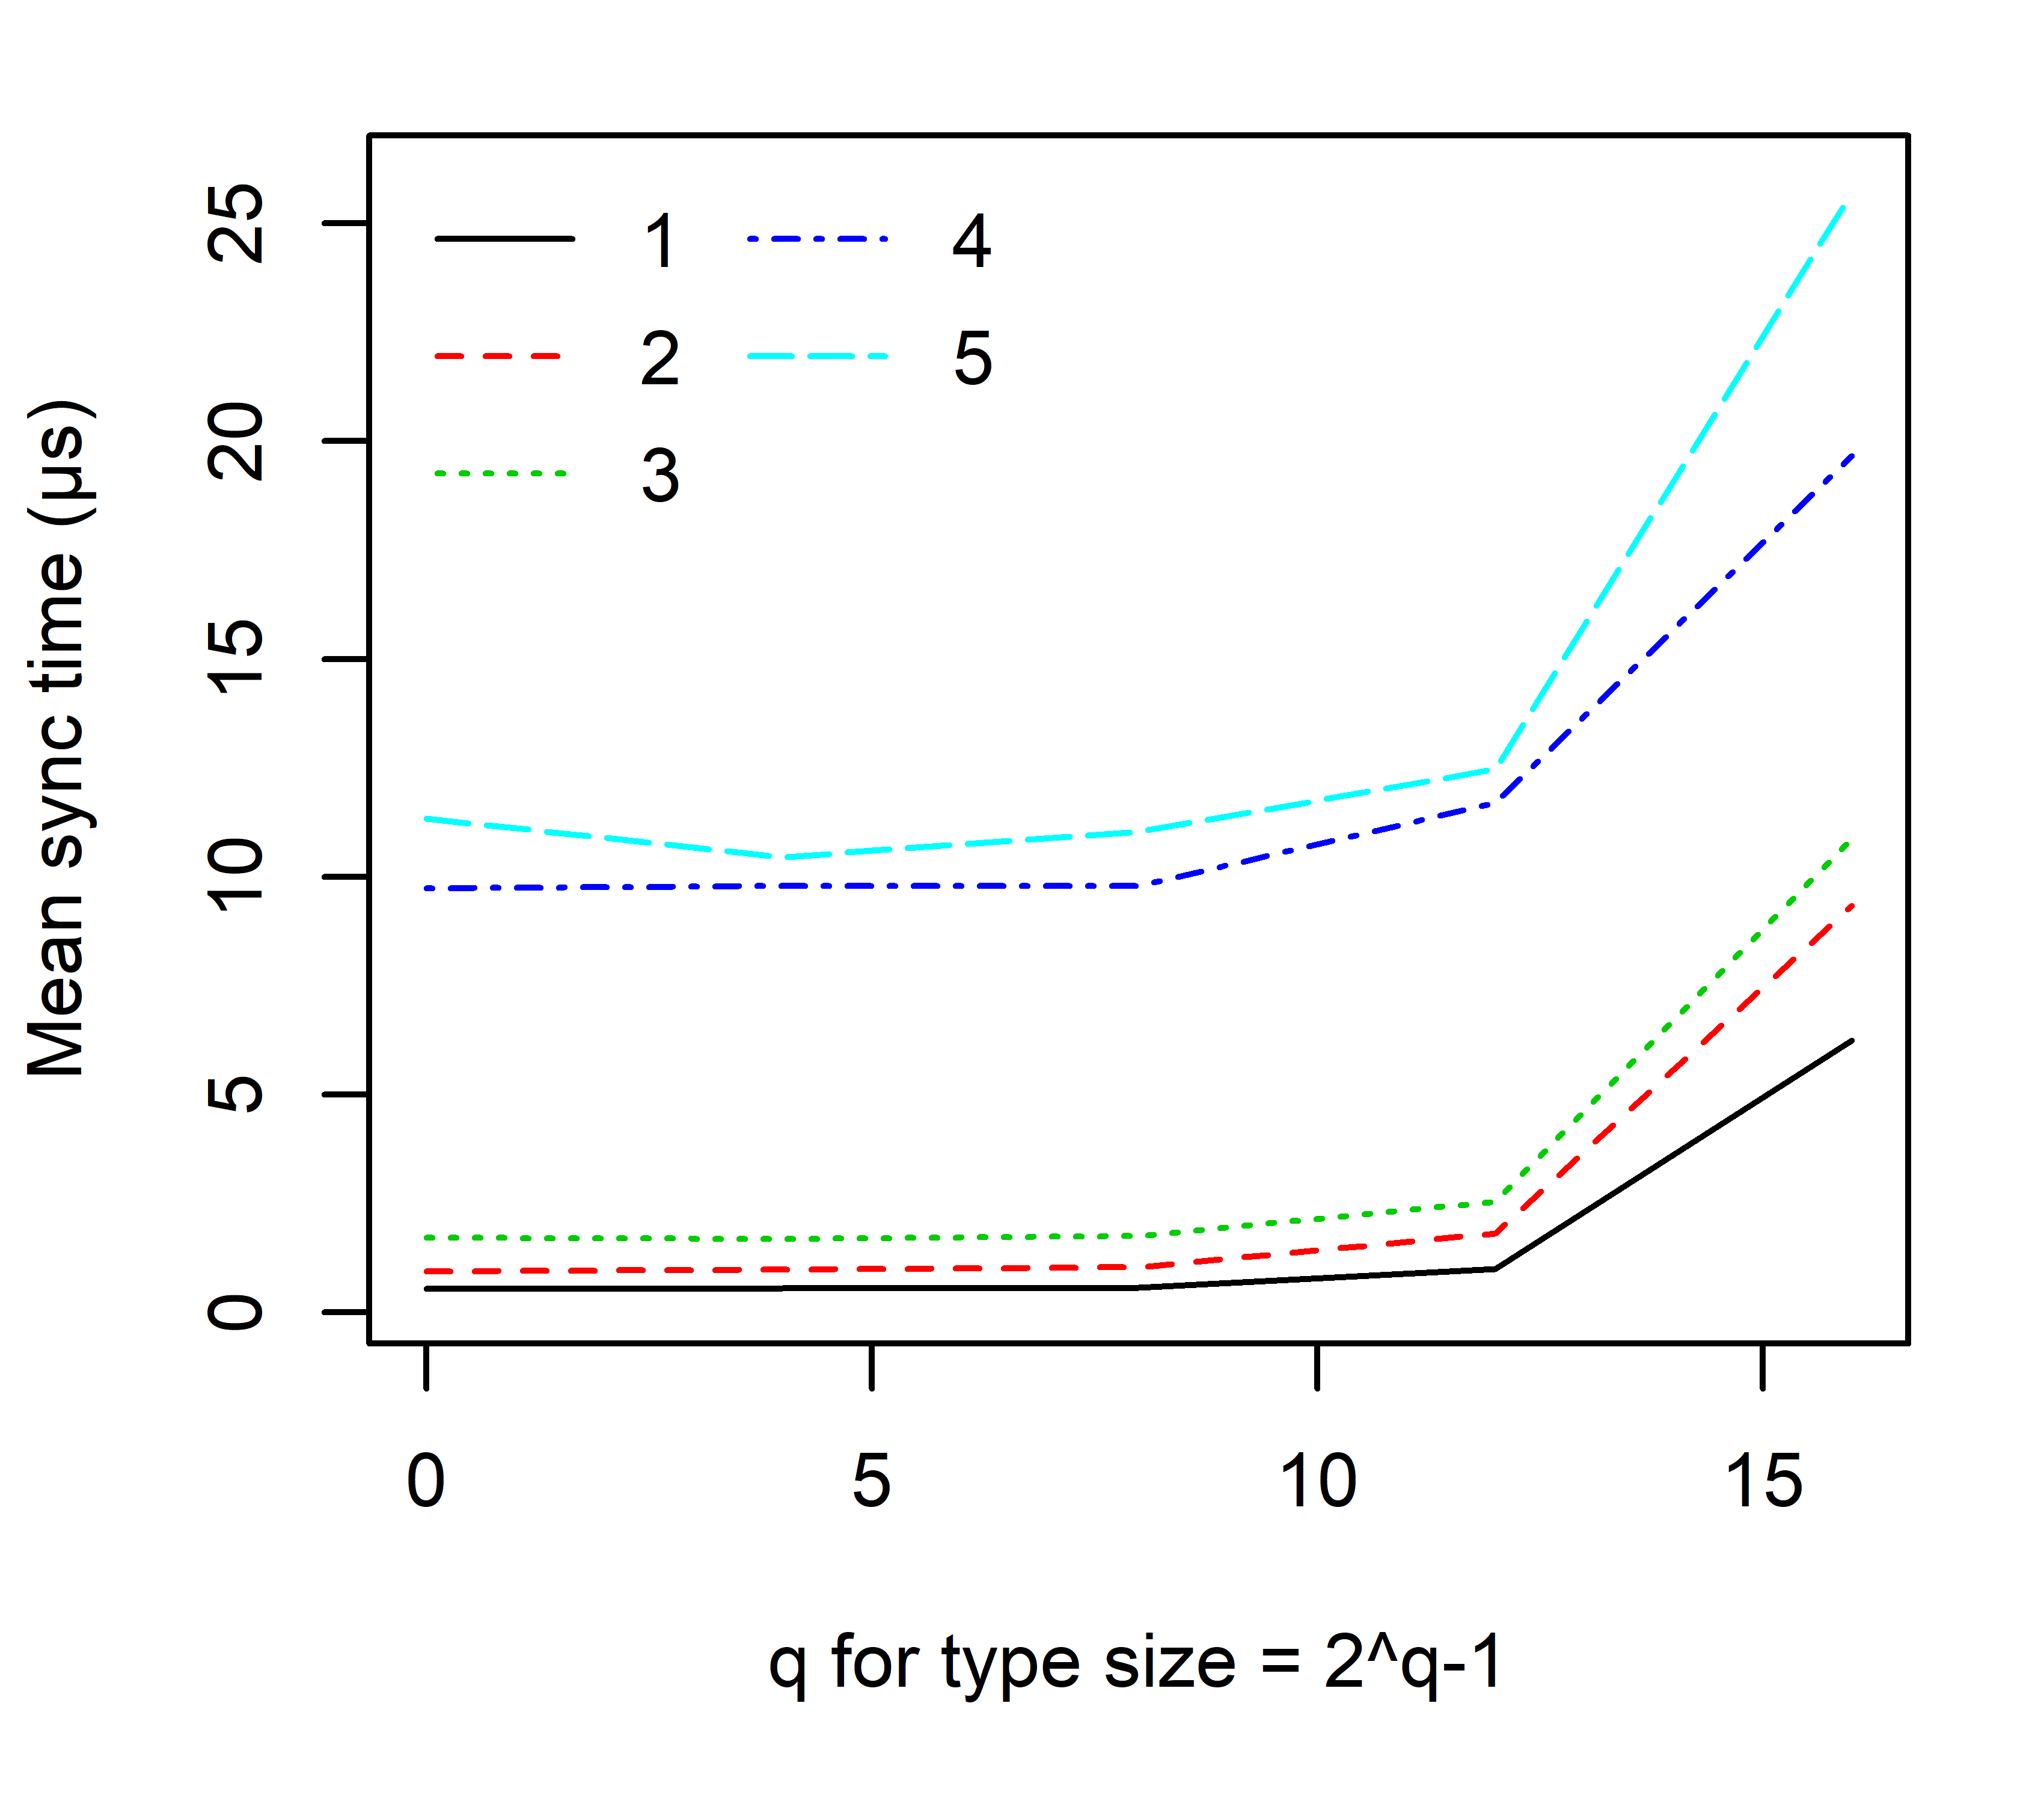
\includegraphics[width=\textwidth]{experiments/simo_copy_0.png}
			\caption{}
			\label{fig:simo_copy_0}
		\end{subfigure}%
		\begin{subfigure}[b]{0.63\textwidth}
			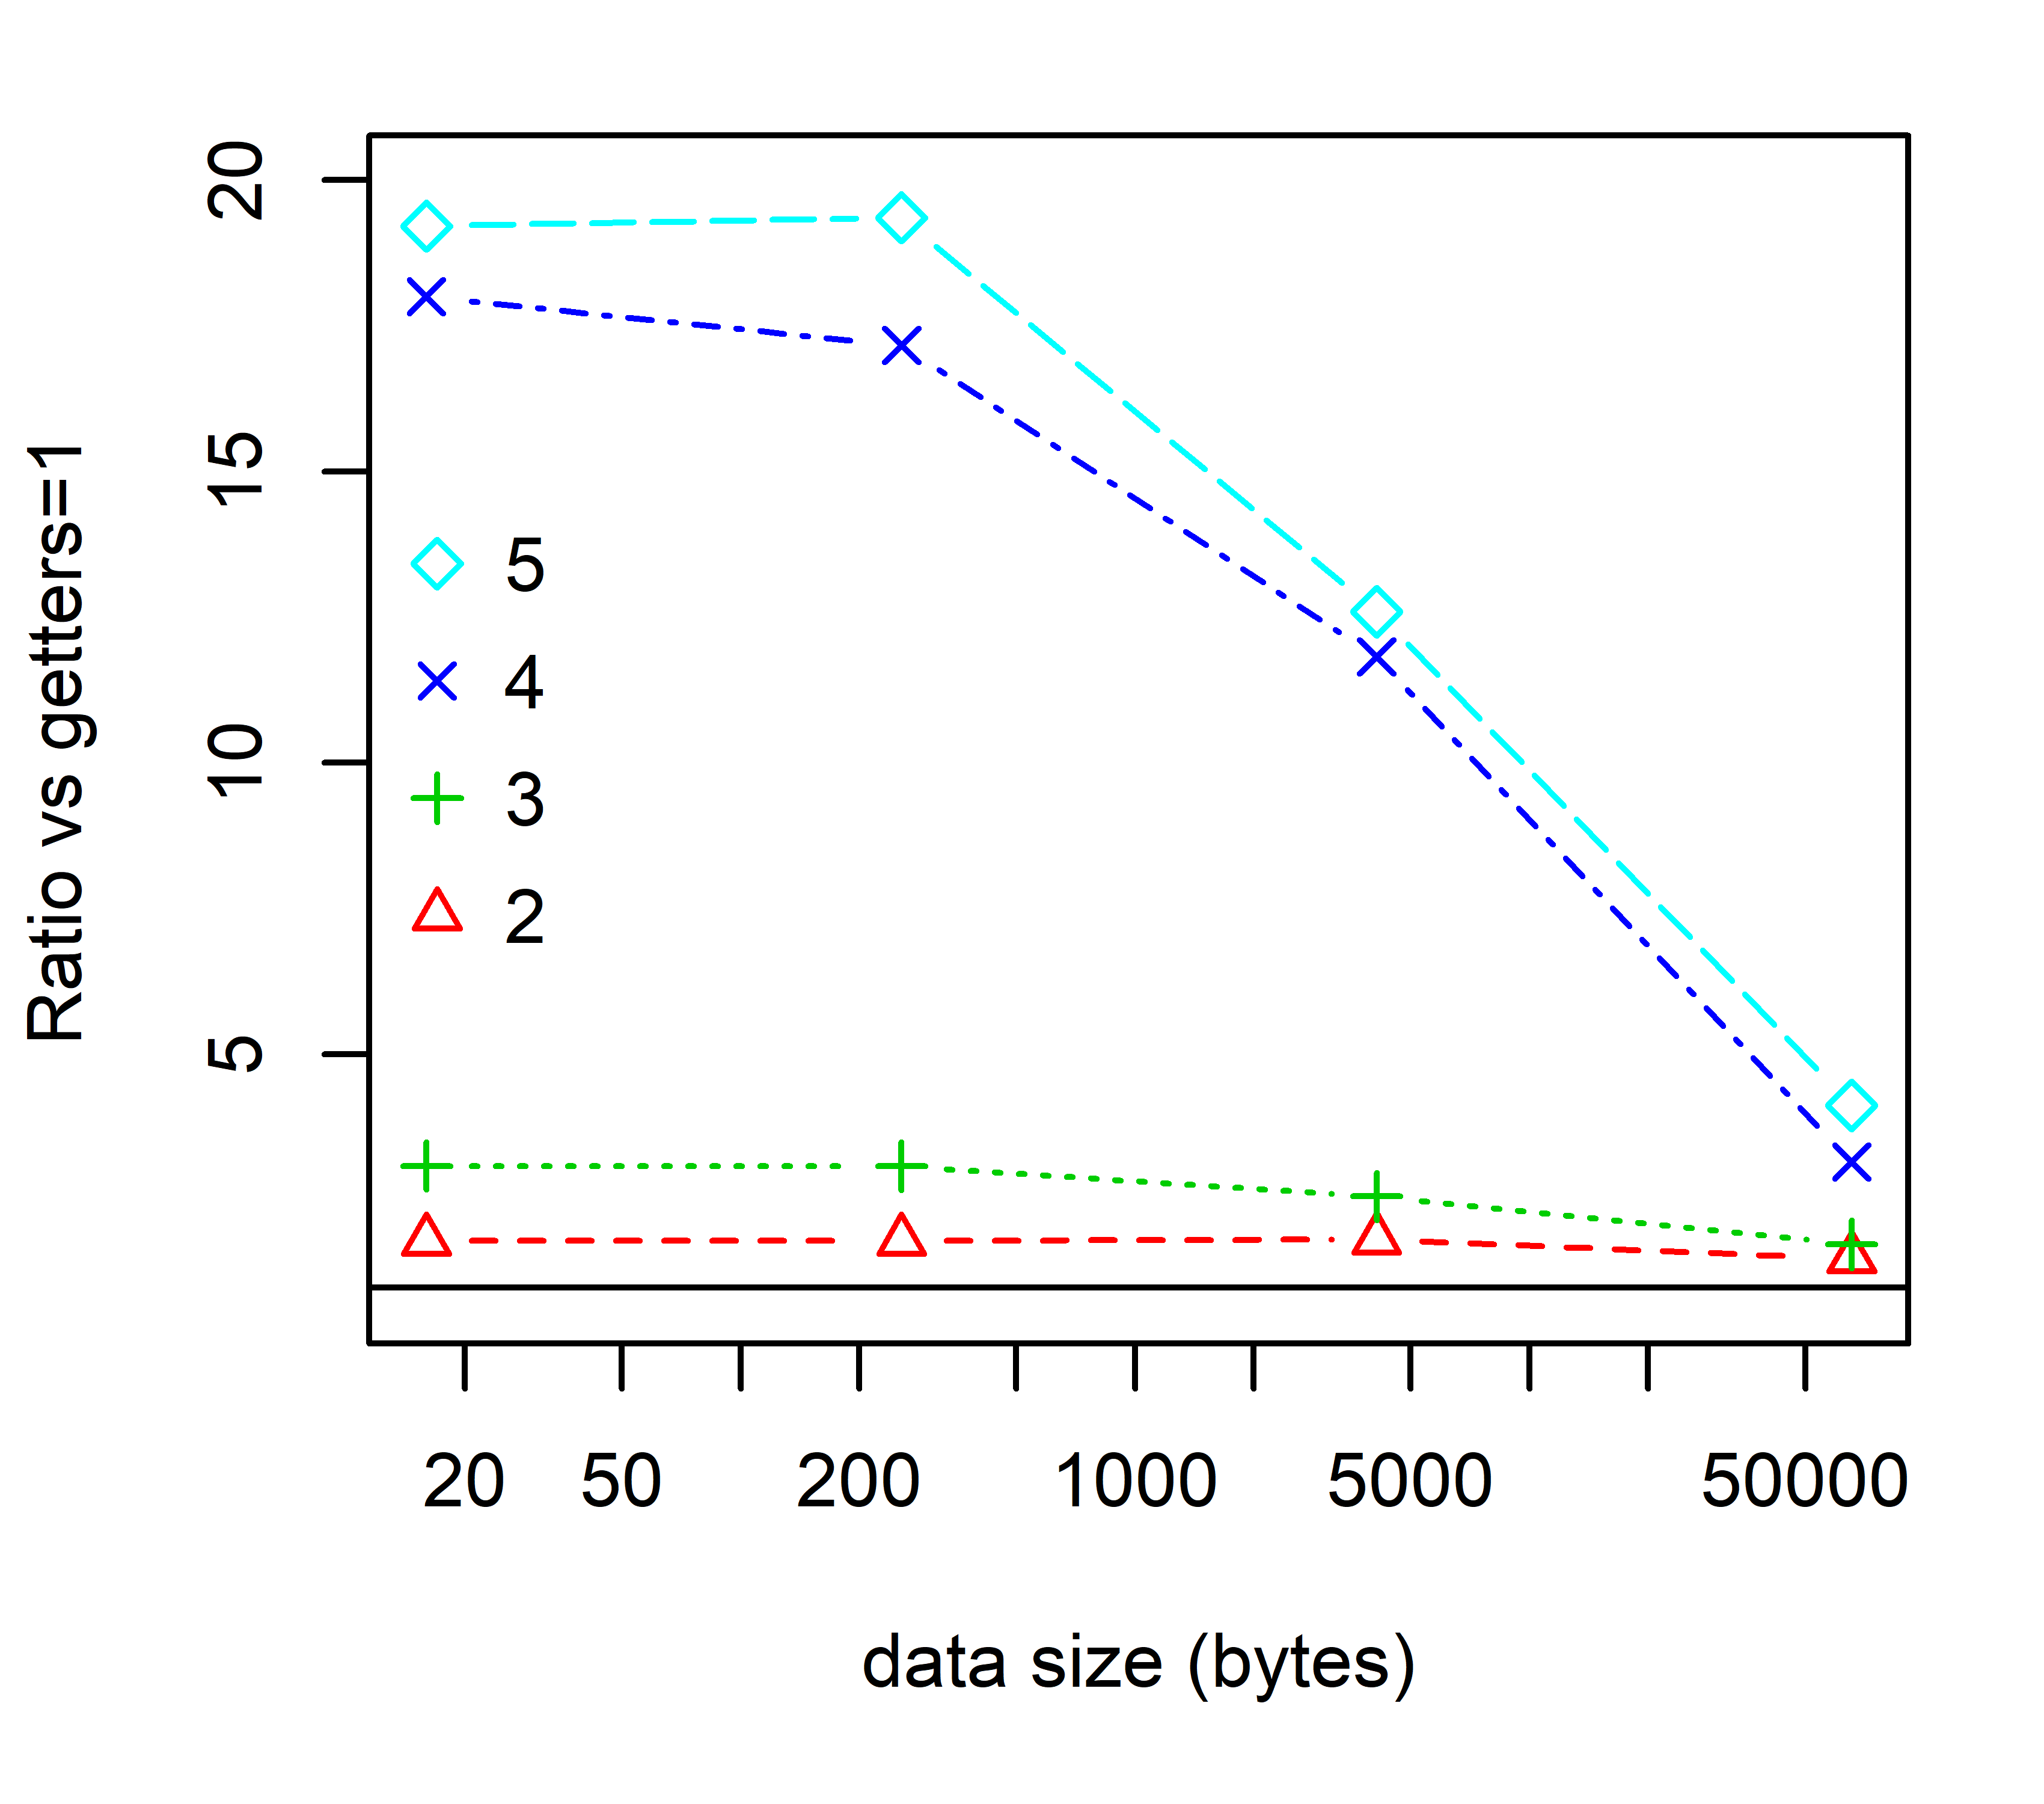
\includegraphics[width=\textwidth]{experiments/simo_copy_1.png}
			\caption{}
			\label{fig:simo_copy_1}
		\end{subfigure}%
	}
	\caption[Synchronization duration for SISO with copy-type data.]{Duration of a synchonization event from the perspective of a putter, putting to a set of getters. The data type implements \code{Copy}, allowing getters to copy the value bit-wise in parallel. Plots show five variants, corresponding to getter sets of sizes one through five, plotted in response to a data type with a changing size in memory.}
	\label{fig:simo_copy}
\end{figure}



The experiment with connector \textit{siso} is shown repeated in Figure~\ref{fig:clone_compete}. This time, the data type is not marked \code{Copy}. Section~\ref{sec:data_exchange} explains how the dissemination of these values to multiple getters are handled, as there are multiple requirements on the order of operations such that correctness can be guaranteed. In this context, Figure~\ref{fig:clone_compete_0} shows that the case of a single getter is exceptionally fast. This is to be expected, as even for non-copy data-types, all but one getter must clone; someone gets the putter's original. These results demonstrate the benefits of this optimization; it is worth noting that invoking a clone also incurs the overhead of an added \textit{virtual function call}.
In this experiment, the cost of \code{clone} was manipulated synthetically as before. As expected, beyond a threshold, the cost of the clone operation dominates, causing runtimes to converge, regardless of the number of getters.



\begin{figure}
	\centering
	\makebox[\textwidth][c]{
		\begin{subfigure}[b]{0.63\textwidth}
			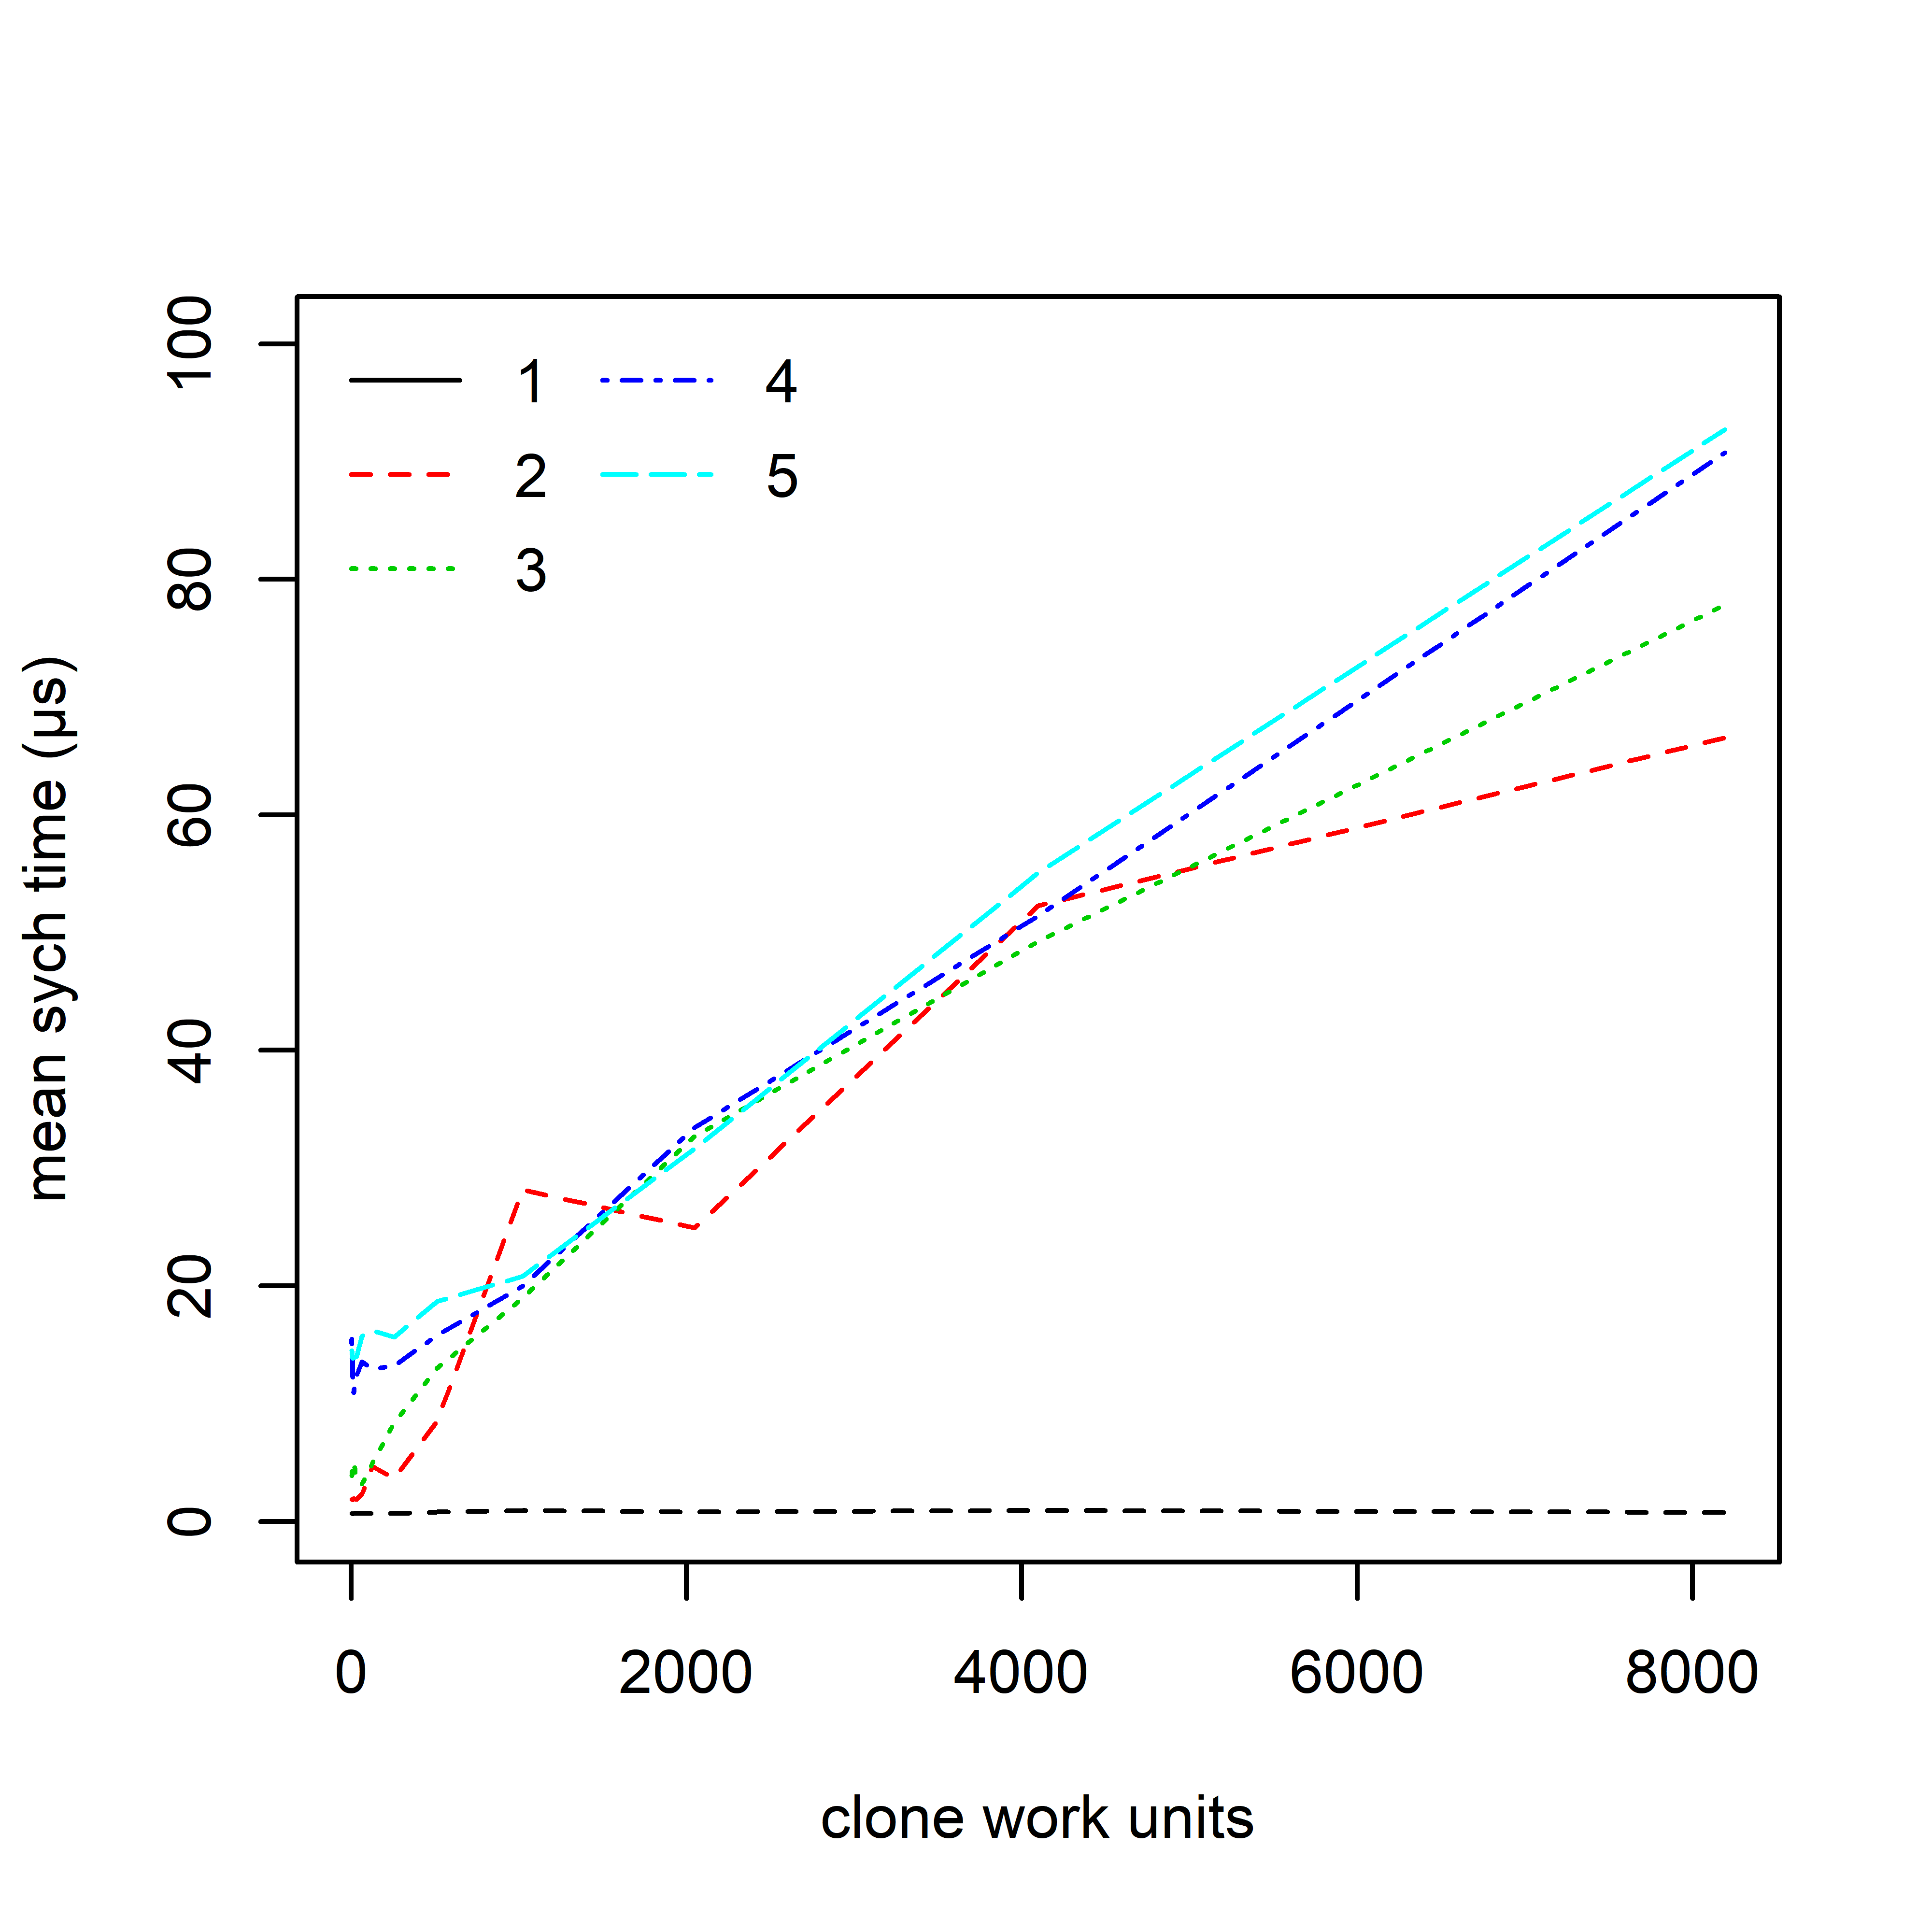
\includegraphics[width=\textwidth]{experiments/clone_compete_0.png}
			\caption{}
			\label{fig:clone_compete_0}
		\end{subfigure}%
		\begin{subfigure}[b]{0.63\textwidth}
			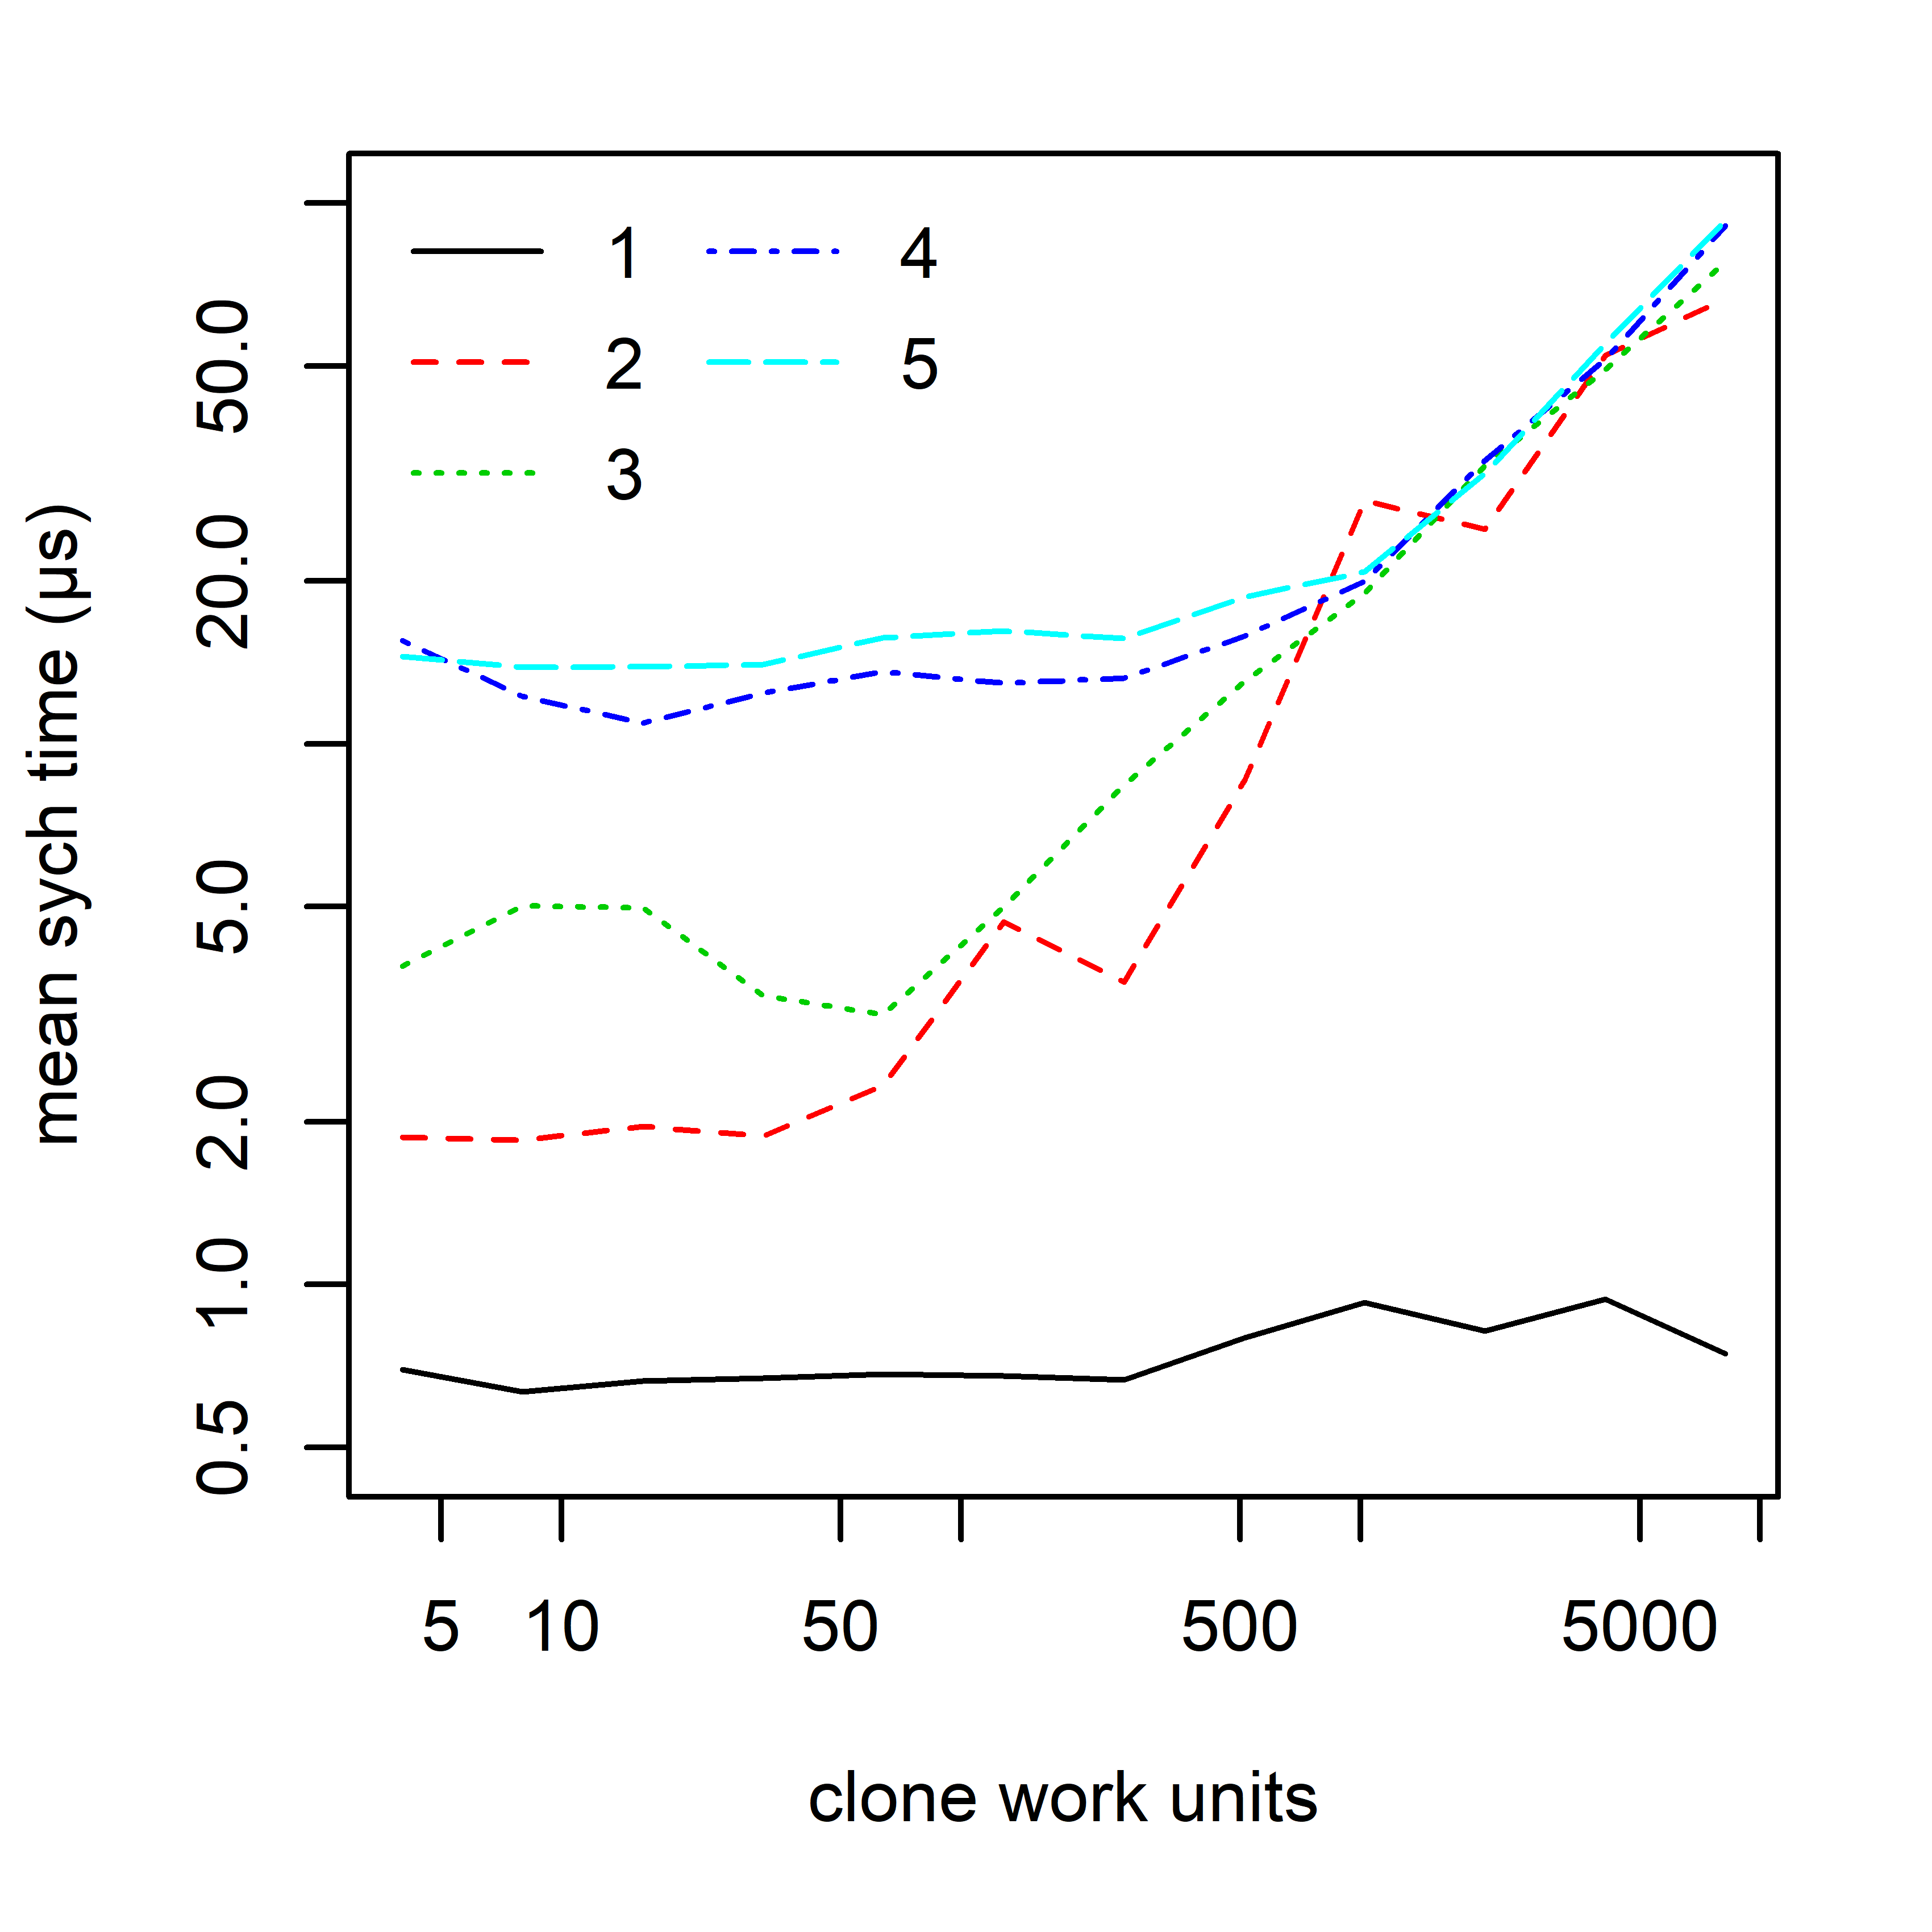
\includegraphics[width=\textwidth]{experiments/clone_compete_1.png}
			\caption{}
			\label{fig:clone_compete_1}
		\end{subfigure}%
	}
	\caption[Duration of interaction in siso connector with clonable data.]{Duration of an interaction in a \textit{siso} connector. Runs are distinguished by the number of getters per interaction with one putter, plotted over an increasingly expensive \code{clone} operation. Figure~(b) repeats the information of (a) to make the subtle differences more visible.}
	\label{fig:clone_compete}
\end{figure}


Figure~\ref{fig:clone_compete_2} omits the exceptional single-getter case to show the effects of competing cloners. Measurements for cheap clone operations differ in runtimes both as a result of increased contention on concurrency primitives, but also as a result of simply having a larger group of getters to wait for, giving more opportunities for stragglers to delay completion. 


\begin{figure}
	\centering
	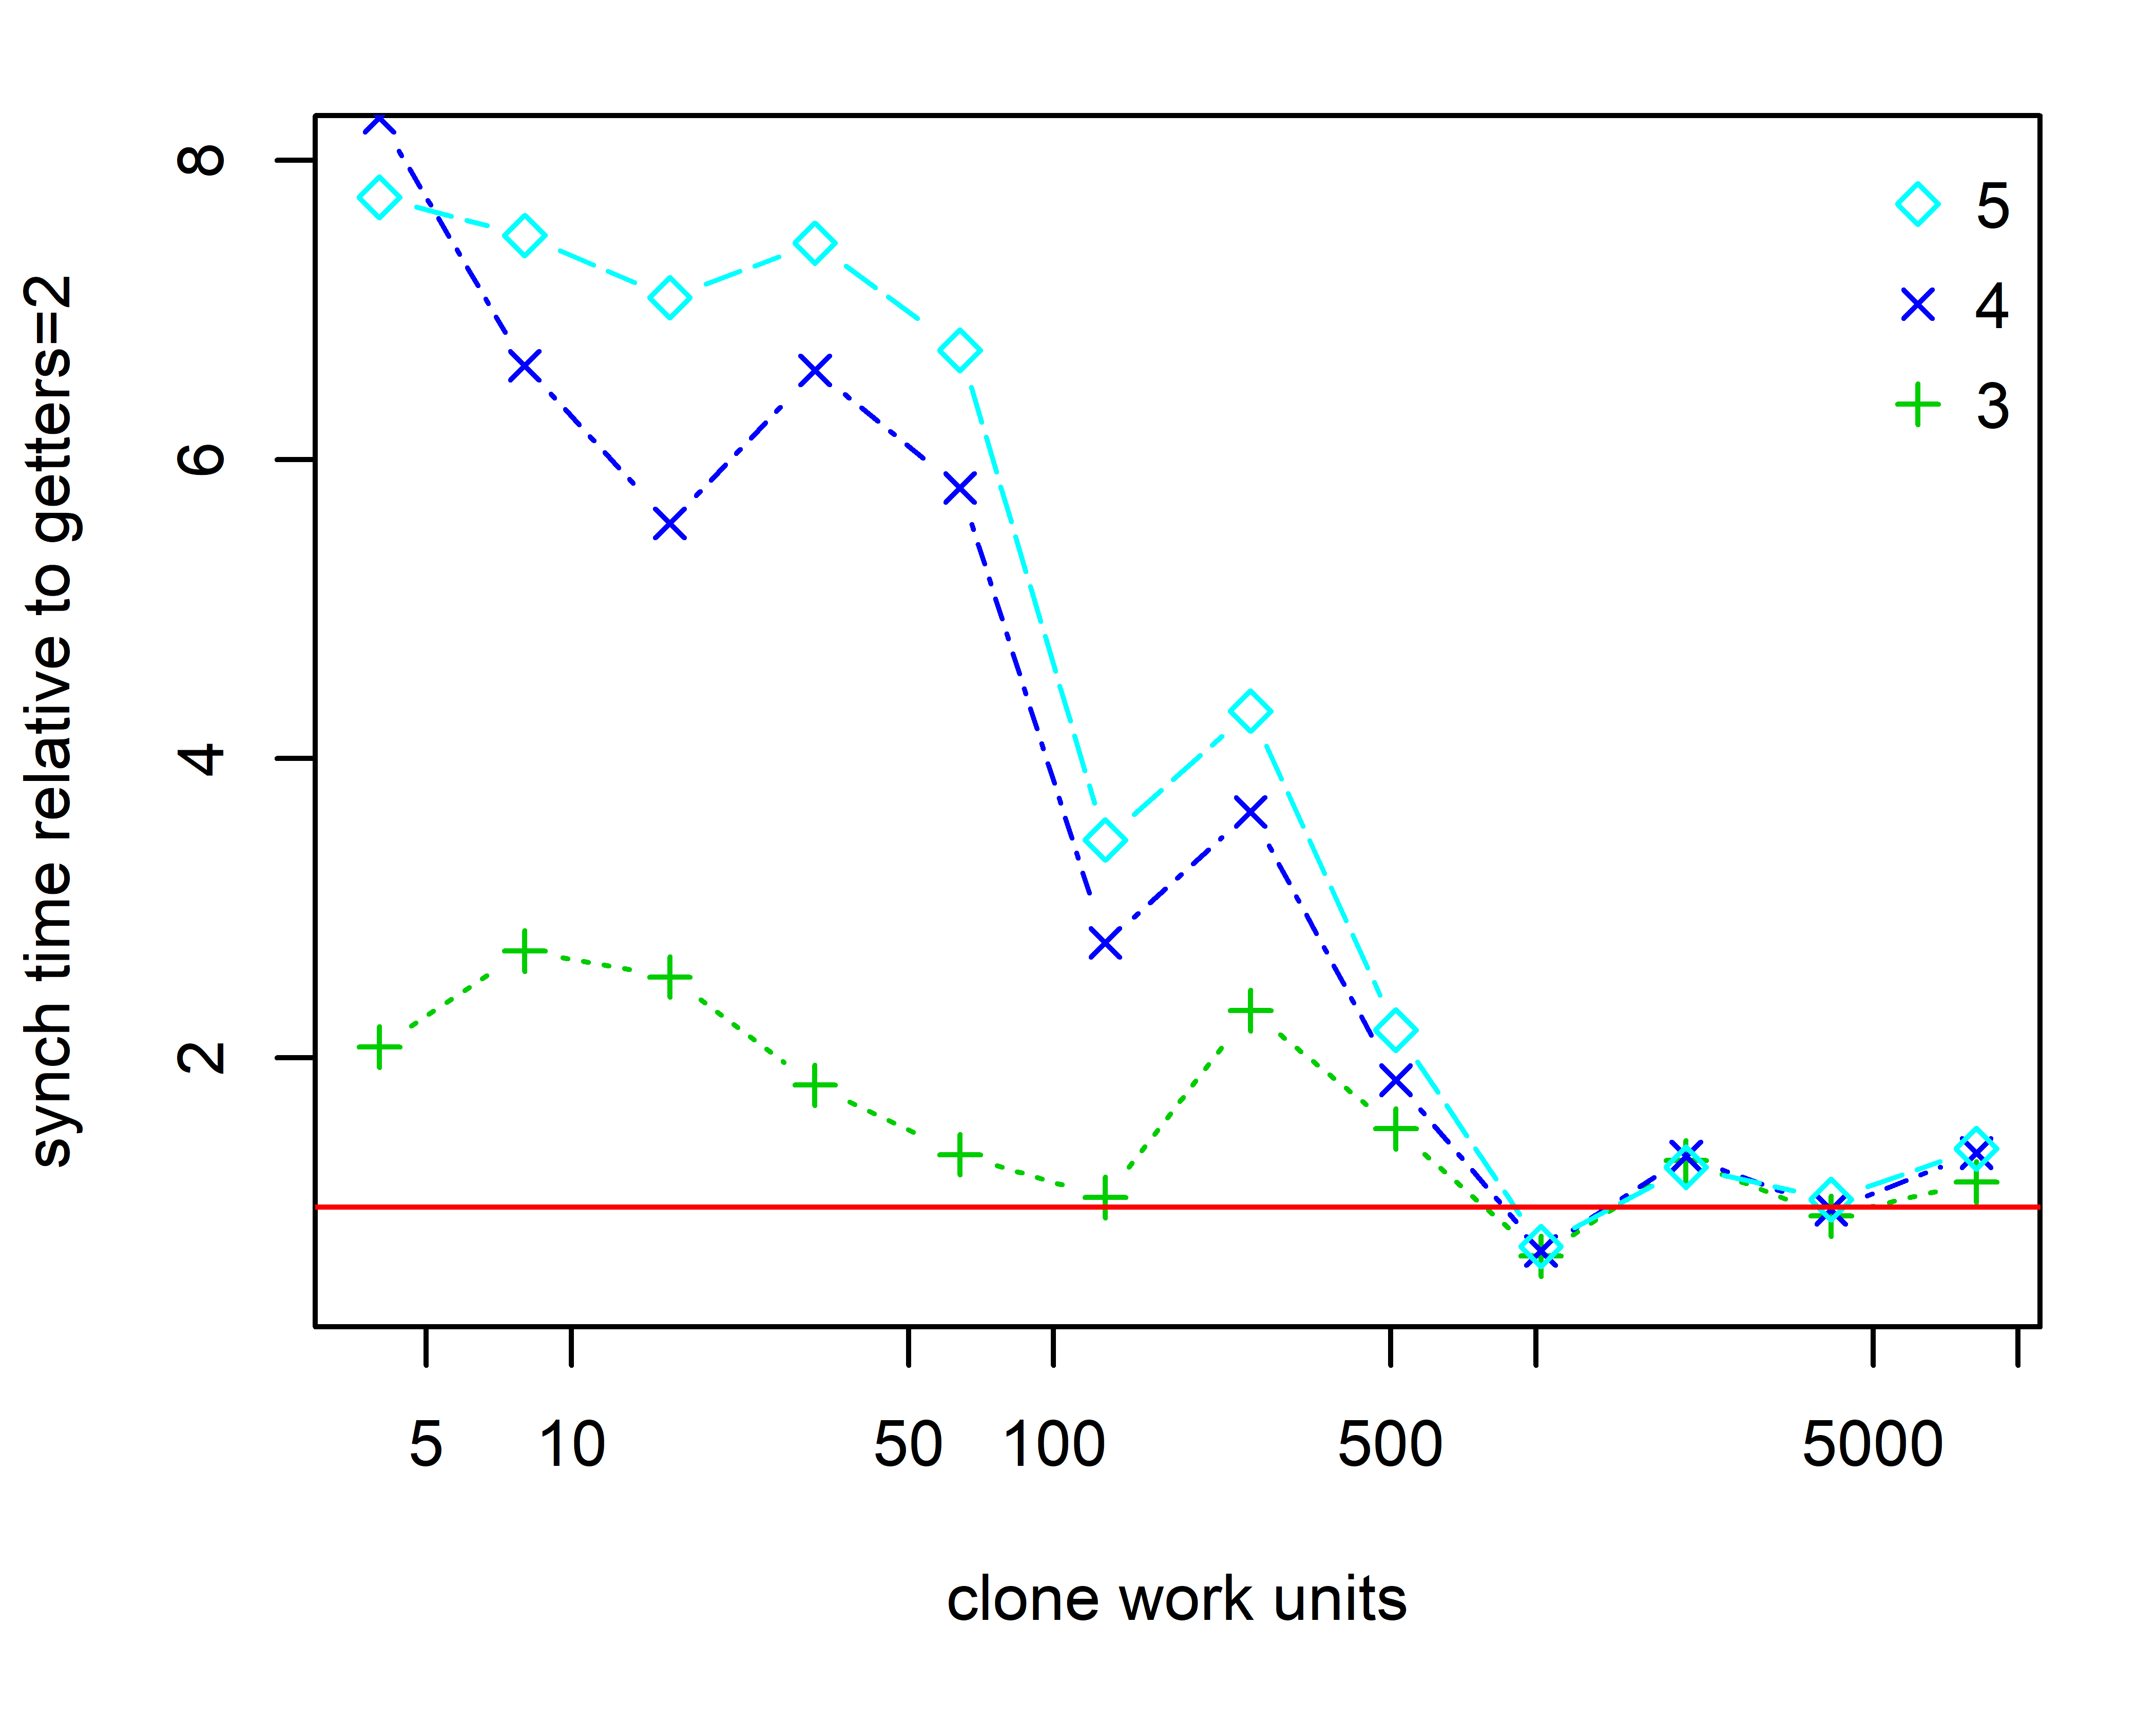
\includegraphics[width=0.80\textwidth]{experiments/clone_compete_2.png}
	\caption[Duration of interaction in siso connector with clonable data plotted relative to the speed of the 2-getter case.]{Measurements of all runs involving the \code{clone} operation from Figure~\ref{fig:clone_compete}, shown plotted relative to that of the case with 2-getters.}
	\label{fig:clone_compete_2}
\end{figure}

TODO getter's point of view in multi-getter siso. check if there is a correlation between \#getters and the MEAN getter RTT

TODO coordinator contention. have N getters that each clone a datum, each firing their own rules. measure mean RTT

TODO update data exchange procedure pseudocode
